\documentclass[grad, numbers]{coppe}
\usepackage[utf8]{inputenc}
\usepackage{amsmath,amssymb}
\usepackage{hyperref}
\usepackage{multirow}
\usepackage{booktabs, multirow} % for borders and merged ranges
\usepackage{glossaries}
\usepackage{soul}% for underlines
\usepackage[table, xcdraw]{xcolor} % for cell colors
\usepackage{changepage,threeparttable} % for wide tables
\usepackage{placeins}

\makelosymbols
\makeloabbreviations

\makeatletter
\renewcommand\tagform@[1]{\maketag@@@{\ignorespaces#1\unskip\@@italiccorr}}
\makeatother

\begin{document}
\title{Previsão de Séries Temporais com Redes Neurais sem Peso}
\foreigntitle{Time Series Forecasting with Weightless Neural Networks}
\author{João Victor}{Almeida Davim}
\advisor{Prof.}{Priscila}{Machado Vieira Lima}{Ph.D.}
\advisor{Prof.}{Leopoldo André}{Dutra Lusquino Filho}{D.Sc.}


\examiner{Prof.}{Nome do Primeiro Examinador Sobrenome}{D.Sc.}
\examiner{Prof.}{Nome do Segundo Examinador Sobrenome}{Ph.D.}
\examiner{Prof.}{Nome do Terceiro Examinador Sobrenome}{D.Sc.}
\department{PESC}
\date{08}{2021}

\keyword{Primeira palavra-chave}
\keyword{Segunda palavra-chave}
\keyword{Terceira palavra-chave}

\maketitle

\chapter*{Dedicatória}
Dedico este trabalho a minha irmã, Carolina, que est\'a começando sua jornada no curso de Direito.

\chapter*{Agradecimentos}

Gostaria de agradecer a todos.

\begin{abstract}

Previsão de séries temporais é um problema presente em diversos cenários do mundo real e, com o início da pandemia de COVID-19, ficou ainda mais evidente a necessidade de extrapolação dos dados para auxiliar nas tomadas de decisão em ações preventivas. Nesse contexto, este trabalho apresenta uma solução agnóstica para o problema de previsão de séries temporais utilizando como modelo de aprendizado de máquina a rede neural sem peso Regression WiSARD, além de empregar técnicas de pré-processamento para transformar a tarefa de previsão de série temporal em um problema supervisionado de regressão. A abordagem proposta se mostrou competitiva em relação à acurácia quando comparada com modelos de destaque na literatura, como Prophet e ARIMA, e obteve melhor desempenho em relação ao tempo de execução e consumo de memória, que podem ser fatores determinantes em cenários de baixa disponibilidade de recursos.

\end{abstract}
\begin{foreignabstract}

Time series forecasting is a problem present in many real-world scenarios and, with the beginning of the COVID-19 pandemic, became even more evident the need for data extrapolation to help decision-making in preventive actions. In this context, this work presents an agnostic solution for time series forecasting using as machine learning algorithm the Weightless Neural Network Regression WiSARD, as well as techniques of pre-processing to transform the task of time series forecasting into a supervised regression problem. The proposed approach was competitive in terms of accuracy when compared with models of high-profile in the literature such as Prophet and ARIMA, and obtained better performance in terms of execution time and memory consumption, which can be determinant factors in low resource availability scenarios.

\end{foreignabstract}
\tableofcontents
\listoffigures
\listoftables
\printlosymbols
\printloabbreviations

\mainmatter
\chapter{Introdução}

Com o início da pandemia da \textit{Coronavirus Disease} (COVID-19) em 2019, surgiram problemas causados pelo descontrole da taxa de transmissão do vírus na população e, portanto, aumentou-se a demanda de soluções para auxílio logístico às medidas médicas, sociais e econômicas. No Brasil, um dos problemas que se destacou no início da pandemia foi o de previsão do número de pessoas infectadas para os próximos dias em cada Estado, que é essencial para a tomada de decisão quanto às medidas preventivas.

No começo da pandemia, a baixa disponibilidade de dados no país foi um desafio que levou ao uso de estratégias alternativas, como o estudo do comportamento das séries temporais de contágio em pandemias passadas ou do cenário atual em países onde o contágio começou antes como China, Itália, Alemanha, França, entre outros. Porém, com a disseminação do vírus, a busca de padrões na curva de infectados começou a se tornar viável, possibilitando caracterizar o problema como um problema de previsão de série temporal univariado.

Assim como o número de infectados, existem outros problemas semelhantes de previsão de séries temporais como previsões meteorológicas, financeiras, de vendas, entre outros. Portanto, generalizando o problema de previsão de séries temporais, e com a objetivo de propor uma alternativa de baixo custo computacional, baixo tempo de resposta e boa acurácia, este trabalho apresenta uma forma de resolver o problema utilizando Redes Neurais sem Peso e técnicas de pré-processamento que transformam o problema de previsão de série temporal em um problema de regressão supervisionado.

As Redes Neurais sem Peso são modelos que apresentam, em geral, tempo de inferência e ajuste menor que a maioria dos modelos, e são excelentes para tarefas que precisam de aprendizado em tempo real. Além disso, o uso de recursos computacionais é baixo, permitindo a sua execução em ambientes computacionais limitados. A utilização dessas redes para resolver o problema de previsão de séries temporais é uma alternativa que também pode viabilizar aplicações em séries temporais com poucas amostras.

A estrutura deste trabalho é a seguinte: o Capítulo~\ref{chap:02} deste trabalho apresenta o problema de previsão de séries temporais e os modelos autoregressivos (ARIMA) e aditivos (Prophet) como duas possíveis soluções, detalhando suas características e apresentando suas implementações. O Capítulo~\ref{chap:03}, por sua vez, introduz o conceito de Redes Neurais sem Peso e seus estimadores de regressão e classificação para problemas supervisionados através do detalhamento do modelo WiSARD e sua adaptação Regression WiSARD. Já as técnicas de pré-processamento para transformação do problema de previsão de séries temporais em um problema de regressão supervisionado são apresentadas no Capítulo~\ref{chap:04}, que, junto com o modelo Regression WiSARD, resolvem o problema de previsão de séries temporais. Além disso, também é apresentado um \textit{piepline} completo de todas as transformações necessárias no pré-processamento para treinamento e inferência do modelo.

O ambiente computacional, as coleções de dados e as métricas de avaliação utilizadas são assuntos abordados no Capítulo~\ref{chap:05}, e são responsáveis por expor a metodologia do trabalho. Além disso, também são apresentados os resultados dos experimentos seguidos de uma breve discussão sobre os mesmos. Finalmente, o Capítulo~\ref{chap:06} recaptula o objetivo, o que foi apresentado, a conclusão dos resultados e os trabalhos futuros.
\chapter{Previsão de Séries Temporais}

\section{Definição do problema de previsão de séries temporais}
Previsão de séries temporais é uma solução adotada para muitos problemas da vida real com o objetivo de, a partir de dados observados, realizar extrapolações para o futuro. Esse tipo de abordagem é muito eficaz quando há poucos dados disponíveis dentro do escopo do problema, pois permite realizar inferências que utilizam dados históricos da própria variável, e podem ser essenciais para o auxílio à tomada de decisão.

Toda previsão de série temporal possui um horizonte de previsão, ou seja, o número de instantes à frente que serão previstos. Esse valor faz parte da caracterização do problema, portanto, é fundamental que todos os ajustes sejam avaliados de acordo com esse horizonte.

Os modelos de previsão podem ser classificados em univariados ou multivariados \cite{box&jenkins}. Modelos univariados utilizam apenas a própria variável como entrada para a previsão, enquanto modelos multivariados, podem utilizar multiplas variáveis para a previsão de uma variável alvo. Quando utilizada a própria variável para a inferência, esta é chamada de endógena, enquanto as restantes são chamadas exógenas.

Existem muitos modelos univariados que são frequentemente utilizados para tarefas de predição de séries temporais. Dentre estes, podem-se citar desde modelos estatísticos como ARMA \cite{box&jenkins} e suas variações \cite{ALZAHRANI2020914} até métodos com modelos aditivos como o Prophet \cite{fbprophet}. Além destes, existem muitos estudos que fazem adaptações de Redes Neurais para esta tarefa como em ZHANG \& QI, 2003 \cite{ZHANG2005501} e até mesmo modelos misturados de Redes Neurais com ARIMA como apresentado em Brockwell \& Davis, 1986 \cite{ZHANG2003159}.

\section{Modelos autoregressivos}
Os modelos utilizados para os experimentos deste trabalho foram escolhidos com base em estudos paralelos realizados com os dados do Covid-19 como em Ribeiro et al., 2020 \cite{RIBEIRO2020109853} e Wang et al., 2020 \cite{WANG2020110058}, e serão descritos nas subseções seguintes com suas respectivas formalizações.
\subsection{ARMA}
O modelo ARMA é uma combinação dos modelos auto-regressivo (AR) e de médias móveis (MA). O modelo auto regressivo puro de ordem $p$, ou seja, $AR(p)$, é formalizado de acordo com a equação \eqref{eq:ar}.

\begin{equation}\label{eq:ar}
    X_{t}=c+\sum ^{p}_{i=1}\rho _{i}X_{t-i}+\varepsilon _{t}\, ,
\end{equation}

onde $\rho _{1}\ldots \rho _{p}$ são os parâmetros, $c$ é uma constante e $\varepsilon _{t}$ representa um ruído branco.

O ajuste de parâmetros a ser realizado na etapa de treinamento do modelo pode ser feito utilizando o método dos mínimos quadrados ou método dos momentos através das equações de Yule-Walker \cite{box&jenkins}.

O modelo de médias móveis (MA) é utilizado junto com o modelo auto regressivo, e é uma abordagem comum para modelagem de séries temporais univariadas \cite{box&jenkins}. Este modelo estabelece uma dependência linear entre os valores atuais da série temporal e os valores passados, e é formalizado de acordo com a equação \eqref{eq:ma}.

\begin{equation}\label{eq:ma}
    X_{t}=\mu+\varepsilon_{t}+\theta_{1} \varepsilon_{t-1}+\cdots+\theta_{q} \varepsilon_{t-q}\, ,
\end{equation}

onde $\mu$ é a média da série, $\theta_{1}, ..., \theta_{q}$ são os parâmetros e $\varepsilon_{t}, ..., \varepsilon_{t-q}$ são os termos do ruído branco.

Cada modelo pode ser utilizado de forma independente, ou em conjunto formando o modelo ARMA. A construção desse modelo se dá pela soma do modelo auto-regressivo com o modelo de médias móveis é expresso na equação \eqref{eq:arma}.

\begin{equation}\label{eq:arma}
    X_{t}=c+\varepsilon_{t}+\sum_{i=1}^{p} \varphi_{i} X_{t-i}+\sum_{i=1}^{q} \theta_{i} \varepsilon_{t-i}\, .
\end{equation}

Existem diversas técnicas para a otimização dos hiperparâmetros $p$ e $q$ para que o modelo seja melhor ajustado aos dados. Uma das formas mais aceitas para encontrar esses valores é o critério de Akaike, conforme recomendado por Peter J. Brockwell e Richard A. Davis em \cite{akaike}.

\subsection{ARIMA}
Alguns problemas de previsão de séries temporais são ligeiramente mais complexos, pois representam uma série temporal não estacionária. Nesse caso específico, o ajuste do modelo ARMA acaba não sendo bom, pois não acompanha a não estacionaridade dos dados. O modelo auto-regressivo integrado de médias móveis (ARIMA) se propõe a resolver o problema da estacionaridade, e pode ser estudado como uma generalização do modelo ARMA.

De forma análoga ao ARMA, os modelos ARIMA são geralmente denotados como $ARIMA(p, d, q)$, onde os parâmetros $p$, $d$ e $q$ são inteiros não negativos que representam a ordem do modelo auto-regressivo (AR), o grau de diferenciação da parte integrada (I) e a ordem do modelo de médias móveis (MA) respectivamente.

A parte integrada do modelo consiste na computação da diferença dos valores atuais da série temporal com os valores subsequentes da mesma. Esse procedimento é realizado $d$ vezes, e este é o parâmetro da parte integrada do modelo. A equação \eqref{eq:arima} descreve o modelo ARIMA.

\begin{equation}\label{eq:arima}
    \left(1-\sum_{i=1}^{p} \phi_{i} L^{i}\right)(1-L)^{d} X_{t}=\left(1+\sum_{i=1}^{q} \theta_{i} L^{i}\right) \varepsilon_{t}\, ,
\end{equation}

em que $X_{t}$ é a série temporal de dados, $t$ é um índice representado por um inteiro, $L$ é o operador de defasagem, $p$ é o hiperparâmetro do modelo auto-regressivo, $q$ é o hiperparâmetro do modelo de médias móveis, $d$ é o número de diferenças da parte integrada, $\phi_{i}$ são os parâmetros do modelo auto-regressivo, $\theta_{i}$ são os parâmetros do modelo de médias móveis e $\epsilon_{t}$ é o ruído branco ou erro aleatório. A estimação de modelos ARIMA é realizada, geralmente, através do método de Box-Jenkins \cite{box&jenkins}, que é um processo iterativo para encontrar os parâmetros que melhor ajustam o modelo aos dados observados.

\subsection{Biblioteca statsmodels}
Os modelos autorregressivos apresentados, são implementados pela biblioteca statsmodels \cite{seabold2010statsmodels}, que é uma biblioteca para análise estatística e econométrica em Python. A biblioteca disponibiliza classes e funções para estimar diferentes modelos estatísticos, como ARMA e suas generalizações, além de testes estatísticos e análise estatística de dados. O pacote possui a licensa de código aberto \textit{Modified BSD (3-clause)}, e sua documentação oficial fica hospedada em statsmodels.org.


\section{Modelo de previsão Prophet}
O modelo de previsão Prophet \cite{fbprophet} foi uma solução criada e adotada pelo Facebook para solução de problemas de previsão no nicho de negócios. A ideia era criar um modelo capaz de utilizar características comuns na maioria dos problemas de previsão para tentar melhorar a acertividade em relação à modelos considerados automáticos como o ARIMA. Então, para facilitar a utilização do modelo por analistas, que na maior parte dos casos, não possui conhecimento detalhado sobre a série temporal que está sendo analisada, o Prophet propõe um modelo que tenha hiperparâmetros intuitivos para alcançar maior escalabilidade no momento da otimização feita pelos analistas.

O modelo é resultado da decomposição da série temporal em 3 principais componentes: tendência, sazonalidade e feriados. Esses componentes compõe o modelo aditivo apresentado na equação \eqref{eq:prophet}.

\begin{equation}\label{eq:prophet}
    y(t) = g(t) + s(t) + h(t) + \epsilon_{t}\, ,
\end{equation}

onde $g(t)$ representa a tendência, $s(t)$ a sazonalidade e $h(t)$ o feriado, e $\epsilon_{t}$ representa o erro não acomodado pelos outros modelos.

\subsection{Modelo de tendência}
Exitem duas implementações do modelo de tendência que podem ser utilizados no Propet. Um é o modelo logístico de saturação, e o outro é o modelo linear.

O modelo de crescimento logístico é, inicialmente, dado por \eqref{eq:logistic_trend}.

\begin{equation}\label{eq:logistic_trend}
    g(t)=\frac{C}{1+\exp (-k(t-m))}\, ,
\end{equation}

onde $C$ é a capacidade de saturação, $k$ é a taxa de crescimento, e $m$ um parametro de deslocamento.

Porém, algumas características são ajustadas para atender melhor aos problema reais de previsão de séries temporais. A capacidade de saturação $C$, por exemplo, pode variar com relação ao tempo sendo substituída por $C(t)$. A taxa de crescimento $k$, também não é constante, então foi introduzido ao modelo um mecanismo de \textit{changepoints}, onde o usuário define um número específico de \textit{changepoints}, que podem ser escolhidos explicitamente ou automaticamente.

Os \textit{changepoints}, são pontos específicos na série temporal onde a taxa de crescimento $k$ pode ser alterada. Dada a sequência de \textit{changepoints} $s_{j}$, $j=1, \ldots, S$ onde $S$ é a quantidade de \textit{changepoints} escolhidos, é definido um vetor de ajuste das taxas $\boldsymbol{\delta} \in \mathbb{R}^{S}$. Cada elemento $\delta_{j}$ desse vetor é somado à taxa constante $k$ de crescimento ao alcançar o changepoint $j$ de forma acumulativa. Sendo assim, a taxa de crescimento pode ser calculada conforme a equação \eqref{eq:growth_rate}.

\begin{equation}\label{eq:growth_rate}
    k+\mathbf{a}(t)^{\top} \boldsymbol{\delta}\, ,    
\end{equation}

onde

\[
    a_{j}(t)= \begin{cases}1, & \text { se } t \geq s_{j} \\ 0, & \text { caso contrário }\end{cases}\, .
\]

Quando a taxa de crescimento é ajustada, é preciso corrigir as conexões entre os segmentos formados pelos \textit{changepoints}, e para tal, é necessário computar um ajuste no parâmetro de deslocamento $j$ conforme mostra a equação \eqref{eq:shift_parameter}.

\begin{equation}\label{eq:shift_parameter}
    \gamma_{j}=\left(s_{j}-m-\sum_{l<j} \gamma_{l}\right)\left(1-\frac{k+\sum_{l<j} \delta_{l}}{k+\sum_{l \leq j} \delta_{l}}\right)\, .
\end{equation}

Portanto, a forma final do modelo de tendência logística é representado pela equação \eqref{eq:final_logistic_trend}.

\begin{equation}\label{eq:final_logistic_trend}
    g(t)=\frac{C(t)}{1+\exp \left(-\left(k+\mathbf{a}(t)^{\top} \boldsymbol{\delta}\right)\left(t-\left(m+\mathbf{a}(t)^{\top} \gamma\right)\right)\right)}\, .
\end{equation}

Para situações onde não é observada saturação no crescimento da série temporal, é recomendado a utilização do modelo de tendência linear. A mesma lógica de \textit{changepoints} também é aplicada nessa situação, e o modelo é dado pela equação \eqref{eq:linear_trend}.

\begin{equation}\label{eq:linear_trend}
    g(t)=\left(k+\mathbf{a}(t)^{\top} \boldsymbol{\delta}\right) t+\left(m+\mathbf{a}(t)^{\top} \gamma\right)\, ,
\end{equation}

onde $k$ é a taxa de crescimento, $\boldsymbol{\delta}$ são as taxas de ajuste (dos \textit{changepoints}), $m$ é o parâmetro de deslocamento e $\gamma_{j}$ assume o valor de $-s_{j}\delta_{j}$ par tornar a função contínua.

\subsection{Sazonalidade}
Muitas séries temporais apresentam características sazonais em diversos períodos, ou seja, podem apresentar comportamento semelhante de hora em hora, dia em dia, semana a semana, e assim sucessivamente. A mesma série pode, inclusive, apresentar mais de uma sazonalidade.

Para flexibilizar o modelo quanto às sazonalidades, são utilizadas séries de Fourier. Portando, o modelo segue a equação \eqref{eq:fourier_seasonality}.

\begin{equation} \label{eq:fourier_seasonality}
    s(t)=\sum_{n=1}^{N}\left(a_{n} \cos \left(\frac{2 \pi n t}{P}\right)+b_{n} \sin \left(\frac{2 \pi n t}{P}\right)\right)\, ,
\end{equation}

onde $P$ é o período da sazonalidade e $\boldsymbol{\beta} = [a_{1},b_{1},\ldots,a_{N},b_{N}]^{\top}$ são os parâmetros ajustados por estimativa.

Para $N=10$, por exemplo, é possível escrever a parte sazonal conforme calculado em \eqref{eq:fourier_seasonality_n_10}.

\begin{equation} \label{eq:fourier_seasonality_n_10}
    s(t)=\left[\cos \left(\frac{2 \pi(1) t}{365.25}\right), \ldots, \sin \left(\frac{2 \pi(10) t}{365.25}\right)\right]\boldsymbol{\beta} \, ,
\end{equation}

onde o parâmetro $\boldsymbol{\beta}$ pode ser estimado considerando $\boldsymbol{\beta} \sim \operatorname{Normal}\left(0, \sigma^{2}\right)$ e o parâmetro $N$ é atribuido empiricamente a $10$ e $3$ para sazonalidades anual e semanal, respectivamente. Essa escolha de parâmetros pode ser automatizada utilizando métodos de seleção de modelos, como o AIC (\textit{Akaike Information Criterion}).

\subsection{Feriados e eventos}
Apesar de não contemplado neste trabalho, o Prophet também inclui um modelo de feriados. O usuário pode fornecer de entrada uma lista de feriados universais ou específicos de seu país. Essa possibilidade permite que seja possível levar em conta os feriados como eventos que influenciam diretamente no comportamento da série temporal, o que é verdade em muitos problemas da vida real.

Para incorporar uma lista de feriados ao modelo, é assumido que o efeito dos feriados são independentes. Portanto, é considerado um conjunto $D_{i}$ de feriados $i$ que ocorrem em diferentes tempos $t$ para construir o vetor

\begin{equation}
    Z(t)=\left[\mathbf{1}\left(t \in D_{1}\right), \ldots, \mathbf{1}\left(t \in D_{L}\right)\right] \, ,
\end{equation}

que multiplicado por um vetor de parametros $\kappa_{i}$, que representa a mudança na série temporal ocorrida em cada feriado forma o modelo de feriados e eventos implementado pelo Prophet:

\begin{equation}
    h(t)=Z(t) \boldsymbol{\kappa}
\end{equation}

Assim como na sazonalidade, para ajustar os parâmetros desse modelo, é considerado $\boldsymbol{\kappa} \sim \operatorname{Normal}\left(0, \nu^{2}\right) .$ Além disso, o modelo também considera datas vizinhas como possíveis candiadatas a desvios no comportamento da série temporal, logo são datas também consideradas como feriado assim como a data marcada como tal.

\subsection{Biblioteca fbprophet}
A biblioteca fbprophet implementa o método Prophet, descrito nessa seção, e disponibiliza uma API em Python e outra em R para sua utilização.\footnote{A documentação fica disponível em $https://facebook.github.io/prophet/docs/quick_start.html$, e é baseada em exemplos.} O pacote possui como conteúdo principal a classe Prophet, que implementa o modelo aditivo completo e recebe os hiperparâmetros em seu construtor. A classe possui 2 métodos principais: o método \textit{fit} para ajustar os parâmetros e o \textit{predict} para fazer as previsões. Ambos recebem os dados de entrada como parâmetro. Além desses métodos principais, existem outros para mostrar gráficos e resultados gerados durante o ajuste e a inferência.

A documentação aborda os hiperparâmetros de cada parte do modelo aditivo, ou seja, tendência, sazonalidade e feriados, além de apresentar como otimizar os hiperparâmetros, evidenciando quais desses devem ser buscados de forma automática e quais devem ser especificados de acordo com os conhecimentos do domínio do problema.

\chapter{Redes Neurais sem Peso} \label{chap:03}
O cérebro humano faz parte do sistema nervoso e é considerado o núcleo de inteligência e aprendizado de um indivíduo. Composto por células nervosas chamadas de neurônios, permite atividades como o controle da ações motoras, integração dos estímulos sensoriais e atividades neurológicas como a memória e reconhecimento de padrões.

As Redes Neurais Artificiais são baseadas em modelos matemáticos e técnicas computacionais inspiradas na estrutura neural dos organismos vivos. Geralmente são compostas por neurônios artificiais interconectados, que aplicam funções no sinal de entrada e alimentam a entrada do próximo neurônio formando uma rede, onde cada neurônio é responsável por parte do processamento da informação. Para cada conexão é atribuído um peso multiplicativo, que é um parâmetro a ser ajustado pelo algoritmo de otimização responsável pelo treinamento.

As Redes Neurais sem Peso possuem neurônios que, ao invés de aplicar funções no sinal de entrada, participam do aprendizado de forma semelhante às memórias de acesso aleatório (RAM). A analogia biológica de tal neurônio é feita com o comportamento excitatório ou inibitório do sinal de entrada da árvore dendrítica. A "força" de um sinal de entrada da árvore dendrítica depende da altura que a conexão sináptica é posicionada, assim como as RAMs decodificam um sinal de entrada binário (excitatório/inibitório) em endereços de memória \cite{briefintrownn}.

As redes neurais sem peso foram inspiradas no classificador de de ênuplas \cite{bledsoe&browning}, que também aplica a decodificação do sinal de entrada para o reconhecimento de padrões. Uma grande aplicação para esse método é o reconhecimento de caracteres. Fotomosaicos com caracteres manuscritos eram representados através de fotocélulas, que por sua vez eram utilizadas como sinal de entrada binário, ou seja, cada fotocélula podia ser estar preenchida ou não formando um padrão binário que representa o caractere e é utilizado para o treinamento do modelo.

A próxima seção explica detalhadamente o processo de codificação tal como descrito pelo parágrafo anterior e a arquitetura de Rede Neural sem Peso utilizada neste trabalho como ponto de partida para o entendimento do modelo de RNSP para previsão de séries temporais.

\section{WiSARD}
A arquitetura do modelo WiSARD (Wilkie, Stonhan and Aleksander Recognition Device) é composta por discriminadores, que são componentes responsáveis pela identidade de uma classe em um problema de classificação supervisionado. Cada discriminador é formado por um conjunto específico de memórias de acesso aleatório (RAMs), que são responsáveis por armazenar o padrão reconhecido no exemplo de entrada. A Figura~\ref{fig:wsd_disc} representa a estrutura da WiSARD seguida abaixo de um de seus discriminadores.

\begin{figure}[!ht]
    \centering
    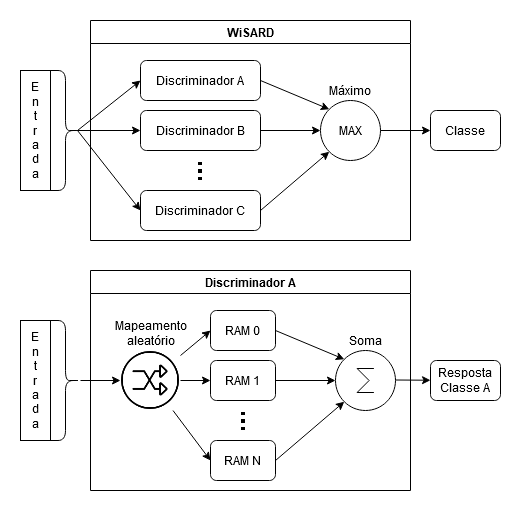
\includegraphics[width=5.0in]{img/wisard_discriminator.png}
    \caption{WiSARD e discriminador. Em caso de empate, o operador máximo seleciona aleatoriamente um dos máximos encontrados.}
    \label{fig:wsd_disc}
\end{figure}

O treinamento de um modelo WiSARD é dado pela escrita nas RAMs de cada discriminador, enquanto a classificação é dada pela leitura dessas posições de memória. A escrita se dá através de um mapeamento aleatório dos bits de entrada em um conjunto de endereços, que serão utilizados para apontar as posições de memória que devem ser escritas, portanto, se faz necessária a utilização de uma entrada binária para a rede. Cada discriminador possui seu próprio mapeamento, que pode ser o mesmo ou não dependendo da implementação. A implementação utilizada neste trabalho, e explicada na Seção~\ref{sec:wisardpkg}, utiliza o mesmo mapeamento para todos os discriminadores.

\begin{figure}[!ht]
    \centering
    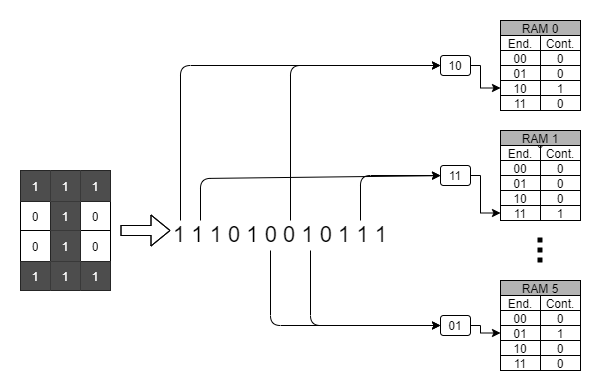
\includegraphics[width=5.0in]{img/wisard_training.png}
    \caption{Treinamento de um exemplo da classe I no seu respectivo discriminador.}
    \label{fig:wsd_train}
\end{figure}

A classificação é realizada lendo-se o conteúdo das RAMs de cada discriminador e comparando a entrada a ser classificada com o conteúdo das RAMs de cada discriminador a fim de descobrir à qual discriminador (ou classe) o exemplo pertence.

\begin{figure}[!ht]
    \centering
    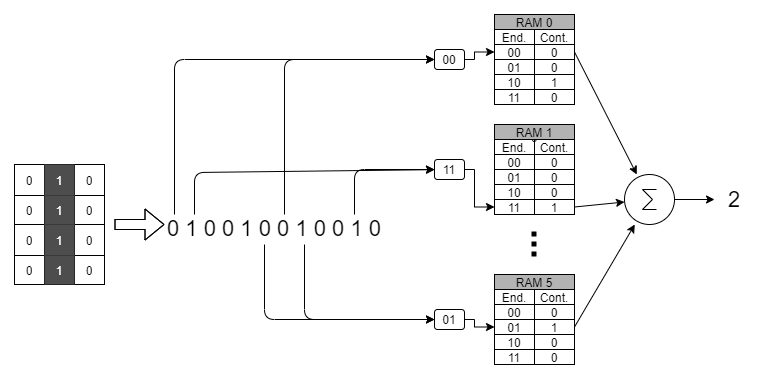
\includegraphics[width=5.0in]{img/wisard_classification.png}
    \caption{Classificação de um exemplo da classe I no seu respectivo discriminador já treinado.}
    \label{fig:wsd_classification}
\end{figure}

Como o modelo requer uma entrada binária tanto para a etapa de treinamento quanto para a entrada de classificação, há uma dependência forte do pré-processamento dos dados a fim de obter uma representação razoável no formato binário, ou seja, transformar os dados de entrada em binário mantendo a capacidade de generalização do modelo. Algumas técnicas de pré-processamento serão apresentadas na Seção~\ref{sec:input_repr}.

Um problema evidente no modelo WiSARD é a possibilidade de empate entre dois ou mais discriminadores, ou seja, mais de um discriminador com a mesma quantidade (máxima) de RAMs que acessaram posições escritas no momento da classificação. Portanto, para contornar tal problema, é utilizada a técnica \textit{bleaching}, introduzida em Grieco et al., 2010 \cite{mentalimages} e primeiramente utilizada como \textit{bleaching} em França et al., 2014 \cite{advanceswns}. A técnica consiste em utilizar as posições de RAM como contadores ao invés de bits, e aplicar um valor limite na saída de cada RAM, de forma que a resposta do discriminador seja a soma do número de RAMs que apresentam o valor acessado superior ao valor limite escolhido como hiperparâmetro. Caso o empate permaneça, o valor de limite é incrementado progressivamente até que ocorra o desempate ou um empate absoluto, ou seja, quando o valor limite ultrapassar o valor do contator de valor máximo.

\begin{figure}[!ht]
    \centering
    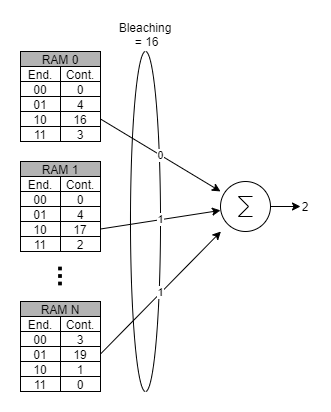
\includegraphics[width=3.0in]{img/bleaching.png}
    \caption{Exemplo de bleaching em um discriminador.}
    \label{fig:bleaching}
\end{figure}

\section{Regression WiSARD}
A tarefa regressão, assim como a de classificação, é uma das tarefas mais abrangentes e divulgadas na área de aprendizado de máquina. Como descrito no capítulo anterior, o modelo WiSARD é utilizado para a resolução de problemas de classificação, mas, como alguns outros modelos de aprendizado de máquina, também pode ser utilizado para problemas de regressão, necessitando apenas de algumas modificações em sua arquitetura.
A principal modificação necessária para utilização da WiSARD para a tarefa de regressão está na estrutura da RAM. Essa adaptação foi proposta por \cite{rew} e se trata de um aumento de dimensionalidade dos valores armazenados em cada posição de memória, ou seja, enquanto na WiSARD cada posição de memória armazena um número inteiro (contador), na Regression WiSARD cada posição de memória armazena 2 valores: o número de acessos e o somatório do valor alvo dos exemplos que acessaram esta posição. A Figura~\ref{fig:ramxram} ilustra a diferença entre as RAMs das duas arquiteturas.

\hspace*{-1.5in}
\begin{figure}[!ht]
    \centering
    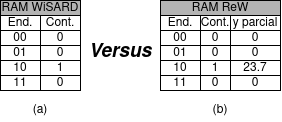
\includegraphics[width=3.0in]{img/ramxram.png}
    \caption{Diferença entre as RAMs das arquiteturas. (a) RAM da WiSARD. (b) RAM da Regression WiSARD.}
    \label{fig:ramxram}
\end{figure}

Para a etapa de treinamento essa é a única mudança necessária. Cada endereço, quando acessado, tem seu contador incrementado em 1 e seu valor incrementado do valor alvo do exemplo que acessou a posição. Já a etapa de inferência, após as RAMs já estiverem preenchidas, o acesso às posições continua sendo feito da mesma forma, porém a resposta do discriminador se torna uma função do contador e do valor das posições de memória acessadas.

\begin{figure}[!ht]
    \centering
    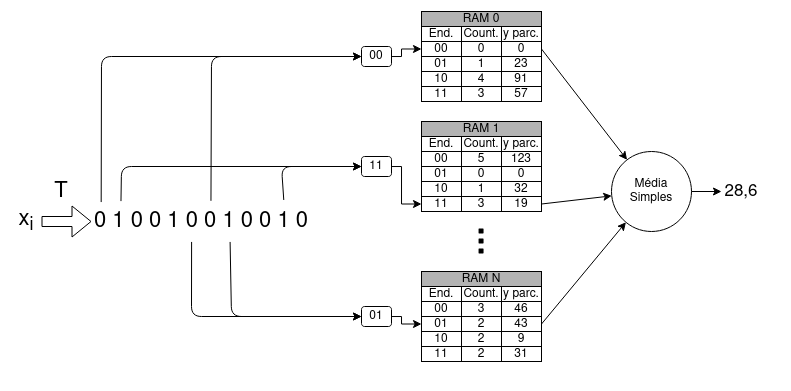
\includegraphics[width=5.0in]{img/rew_regression.png}
    \caption{Discriminador na etapa de inferência da Regression WiSARD transformando a entrada com a função T e agregando o valor de inferência com a função média simples.}
    \label{fig:rew_discr}
\end{figure}

O exemplo da Figura~\ref{fig:rew_discr} mostra o discriminador utilizando uma média simples como função dos valores da posição de memória acessada. É bem intuitivo e coerente pensar que essa função pode variar de acordo com o problema e ser tratada como um hiperparâmetro do modelo. Alguns exemplos de funções utilizadas são a média simples, mediana, média harmônica e média geométrica \cite{rew}.

Além da função de agregação, é fato a permanência da necessidade de transformação da entrada para valores binários na Regression WiSARD. Para tal, existem diferentes técnicas de binarização que serão apresentadas na Seção~\ref{sec:input_repr}.

\section{Representação da entrada} \label{sec:input_repr}
Tanto a WiSARD quanto a \textit{Regression} WiSARD possuem como requisito a representação binária da entrada. Como grande parte dos problemas do mundo real não são representados de forma binária, então é imprescindível a utilização de uma técnica de binarização que minimize a perda de informação para o modelo. Existem diversas técnicas já desenvolvidas que possuem vantagens e desvantagens quando utilizadas como preprocessamento para o treinamento de RNSPs, como o Limiar, a Transformação Termômetro, Filtro de \textit{Marr–Hildreth}, Filtro Laplaciano, entre outros. Um estudo comparativo de tais métodos pode ser encontrado em Kappaun et al., 2016 \cite{binenctec}.

Para o escopo desse trabalho, será utilizada a transformação Termômetro, que possui as características necessárias para garantir um bom desempenho da rede. A transformação recebe 3 parâmetros: tamanho (\textit{sz}), valor mínimo (\textit{min}) e valor máximo (\textit{max}). O tamanho é a quantidade de bits que é utilizada para representar 1 número real, enquanto o valor mínimo e máximo representam o menor e o maior valor real possível assumido respectivamente. O algoritmo da transformação termômetro consiste na divisão do espaço entre o mínimo e o máximo em \textit{sz} pedações de mesmo tamanho, atribuindo um valor limite para cada uma das divisões. Em seguida, cada pedaço é preenchido por um bit 1 ou 0 dependendo se o valor que está sendo transformado está acima ou abaixo do valor limite. A Figura~\ref{fig:therm_ex} ilustra um número inteiro antes e após a transformação termômetro.

\begin{figure}[!htp]
    \centering
    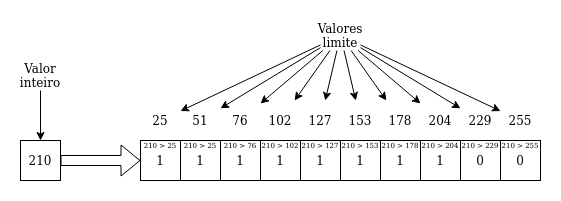
\includegraphics[width=5.0in]{img/therm_example.png}
    \caption{Exemplo de transformação termômetro do número 210}
    \label{fig:therm_ex}
\end{figure}

É importante evidenciar que as técnicas utilizadas acima são fundamentais. A transformação dos números em binário modificando sua base de 10 para 2 tem um problema crucial. Ao mudar a base, os números perdem a propriedade de proximidade na representação, o que dificulta o processo de aprendizado da rede. Por exemplo, os números 11 e 12 possuem uma representação bem diferente quanto transformados da base 10 para 2, quando na verdade, deveriam ter representações próximas, pois são números próximos. A transformação termômetro garante essa propriedade.

\section{Biblioteca wisardpkg} \label{sec:wisardpkg}
Quase todos os métodos descritos nas seções anteriores, incluindo as RNSPs WiSARD e Regression WiSARD, são implementados na biblioteca wisardpkg \cite{wisardpkg}.

A documentação da biblioteca fica hospedada no GitHub em \url{https://iazero.github.io/wisardpkg}, e o repositório pode ser acessado em \url{https://github.com/IAZero/wisardpkg}. Os modelos são implementados em C++, mas também podem ser utilizados em Python através da dependência pybind11.

A biblioteca é multiplataforma, podendo ser utilizada nos sistemas operacionais Windows, Mac OSX ou Linux. Para Python é distribuída através do repositório de pacotes Pypi, e em C++ deve ter o código fonte e cabecalho incluídos no projeto.

Os dois principais módulos da biblioteca são os de Modelos (models) e Binarização (binarization), dando suporte para o treinamento dos modelos WiSARD e para o pré-processamento necessário para transformar o input em binário, como o método termômetro descrito na seção \ref{sec:input_repr}.
\chapter{Autoregressão com WiSARD}
Como previsto no capítulo de redes neurais sem peso, o modelo Regression WiSARD é utilizado para resolver problemas de regressão, porém não é possível realizar previsão de séries temporais por depender de características que não são função do tempo. É possível, entretanto, tratar um problema de previsão de séries temporais como um problema de regressão aplicando técnicas como a janela deslizante e médias móveis conforme detalhado nas seções seguintes.

\section{Janelas deslizantes}
O método de janelas deslizantes é essencial para a Regression WiSARD ser capaz de realizar previsões de séries temporais. Isso ocorre porque é a técnica que permite transformar o problema temporal em um problema de regressão supervisionado.

O método consiste em tornar cada amostra dependente das N amostras anteriores, e faz isso alocando uma janela de N amostras no início da série temporal e deslocando até o final de amostra em amostra para formar a matriz de características, conforme ilustra a Figure~\ref{fig:sliding_window}.

    % \begin{figure}[!ht] \label{fig:sliding_window}
    % \centering
    % \includegraphics[width=5.0in]{img/}
    % \caption{Legenda}
    % \end{figure}
% Exemplos práticos de utilização...

% Como ajuda na previsão de séries temporais com a Regression WiSARD...
\section{Média móvel}


% Exemplos práticos de utilização...

% Como ajuda na previsão de séries temporais com a Regression WiSARD...
\section{AutoRegression WiSARD}
% Explicar treinamento do modelo...

% Explicar predições com o modelo...

% Aprendizado em tempo real...

\chapter{Avaliação Experimental}
\label{chap:05}

Todos os experimentos realizados nesse trabalho foram reproduzidos para as coleções de dados referentes ao número de casos confirmados de COVID-19 no Rio de Janeiro, temperatura mínima diária em Melbourne e dados gerados por um processo determinístico. Os experimentos consistem no treinamento dos modelos ARIMA, Prophet e Regression WiSARD e avaliação de acordo com as métricas de acurácia, tempo e custo computacional (uso de memória RAM). Em todos os casos, foram reservadas as 7 observações finais de cada \textit{dataset} para avaliação quanto às métricas de acurácia e tempo de ajuste.

\section{Ambiente computacional}
Para os experimentos realizados neste trabalho, foram utilizados 2 máquinas com configurações diferentes de hardware. Uma delas possui o hostname poseidon e está hospedada nas dependências do Laboratório de Arquitetura de Computadores e Microeletrônica (LAM), enquanto a outra trata-se de um notebook pessoal com hostname jvdvostro. O servidor poseidon foi utilizado para realizar a busca de hiperparâmetros, pois é a etapa que mais consome recursos computacionais. O jvdvostro foi utilizado para coletar as métricas de inferência, gerar gráficos e fazer a análise dos resultados. A Tabela~\ref{tab:hardware} expõe as configurações de \textit{hardware} de ambos computadores utilizados nos experimentos.

\begin{table}[!htp]
    \caption{Configurações de \textit{hardware} dos computadores.}
    \label{tab:hardware}
    \setlength\extrarowheight{5pt}
    \centering
    \begin{tabular}{|c|c|c|c|}
        \hline
        \rowcolor[HTML]{C0C0C0}
        Hostname  & CPU                           & RAM   & Sistema Operacional \\ \hline
        jvdvostro & Intel i7-5500U (4) @ 3.000GHz & 8 GB  & Arch Linux x86\_64  \\ \hline
        poseidon  & Intel i7-6700 (4) @ 3.40GHz   & 32 GB & Ubuntu Linux        \\ \hline
    \end{tabular}
\end{table}

Os experimentos foram realizados utilizando \textit{scripts} e \textit{notebooks} Python, dependendo da etapa e da finalidade. Para a busca de hiperparâmetros e avaliação dos modelos em relação ao erro, foram utilizados \textit{scripts}, enquanto para a avaliação de métricas de tempo de inferência e uso de memória foram utilizados \textit{notebooks}.

\section{Coleções de dados}
Foram utilizadas para os experimentos deste trabalho 3 coleções de dados. Dentre estas, duas foram coletadas de fontes públicas abertas na internet e uma foi gerada artificialmente. Todas foram armazenadas em disco local no formato tabular com extensão csv (\textit{comma separated values}). O número de casos confirmados de COVID-19 no Rio de Janeiro foi o primeiro dataset utilizado nos experimentos e serviu como um dos motivadores do estudo realizado. A temperatura mínima diária em Melbourne e os dados gerados sintéticamente serviram como prova de conceito para averiguar a eficiência dos métodos aplicados em diferentes cenários, portanto foram submetidos aos mesmos métodos e técnicas aplicados na primeira coleção de dados. As duas coleções de dados retiradas de fontes públicas possuem licensa que permite a sua utilização para fins acadêmicos, e podem ser consultadas nos endereços disponibilizados nesta Seção.

\subsection{Casos confirmados de COVID-19 no Rio de Janeiro} \label{subsec:casos_confirmados}
Com o auxílio da biblioteca \textit{requests} do Python, foi criado um \textit{script} para baixar e armazenar localmente o número de casos confirmados de COVID-19 no Estado do Rio de Janeiro. O arquivo csv foi baixado diretamente do web site da Secretaria de Saúde do Estado do Rio de Janeiro. \footnote{$http://sistemas.saude.rj.gov.br/tabnetbd/dhx.exe?covid19/covid_munic_diario.def$} Para manter a reprodutibilidade dos experimentos, o período analisado foi congelado entre as datas 01/01/2020 e 04/07/2021. A Figura~\ref{fig:casos_confirmados} mostra um gráfico da série temporal não acumulada do número de casos confirmados diário, ou seja, os valores absolutos de casos registrados em cada dia sem considerar os dias anteriores.

\begin{figure}[!htp]
    \centering
    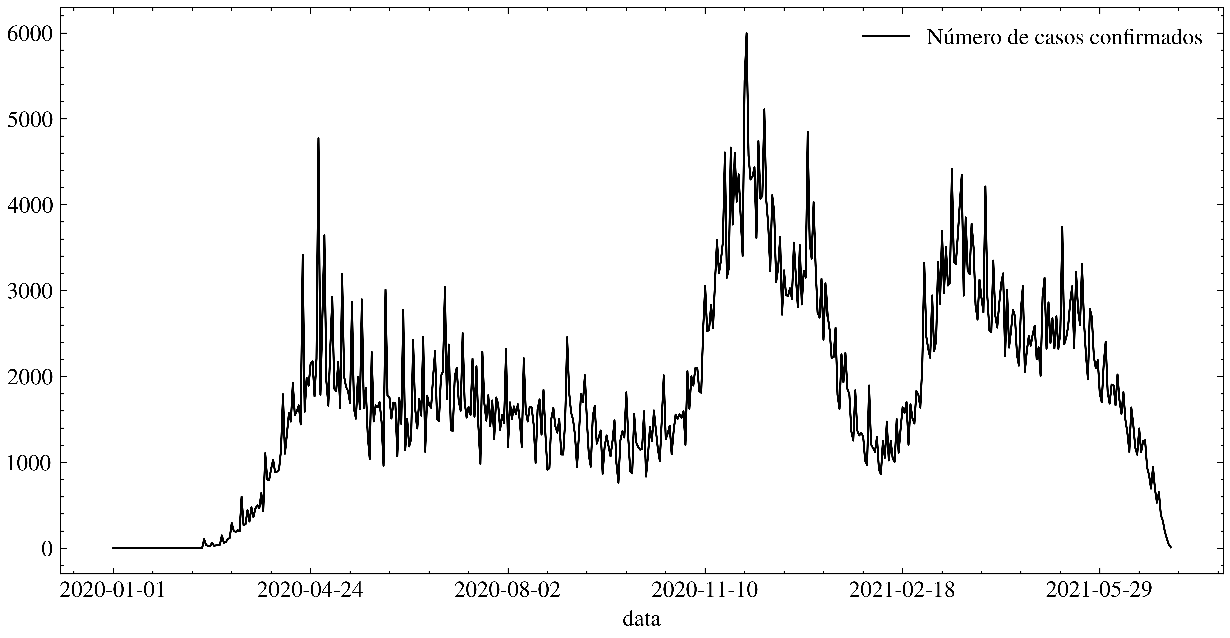
\includegraphics[width=5.0in]{img/casos_confirmados.pdf}
    \caption{Série temporal do número de casos confirmados de COVID-19 no Rio de Janeiro.}
    \label{fig:casos_confirmados}
\end{figure}

A Figura~\ref{fig:casos_confirmados} mostra que há flutuações a curto pazo, que podem ter sido geradas por diversos fatores na coleta dos dados, como, por exemplo, a subamostragem. Como a coleta dos dados utilizados foi feita de fontes externas e públicas, os experimentos deste se limitaram a trabalhar com o dado como foi disponibilizado, sem aprofundar na avaliação da coleta. Porém, para remover a influência dessas flutuações, foi aplicado o método de médias móveis variando o parâmetro do número de amostras junto à busca de hiperparâmetros para encontrar o melhor ajuste. A Figura~\ref{fig:casos_confirmados_ma} mostra a mesma série temporal com as médias móveis em vermelho considerando-se o parâmetro $n=7$ como exemplo de suavização na flutuação dos valores da série temporal.

\begin{figure}[!htp]
    \centering
    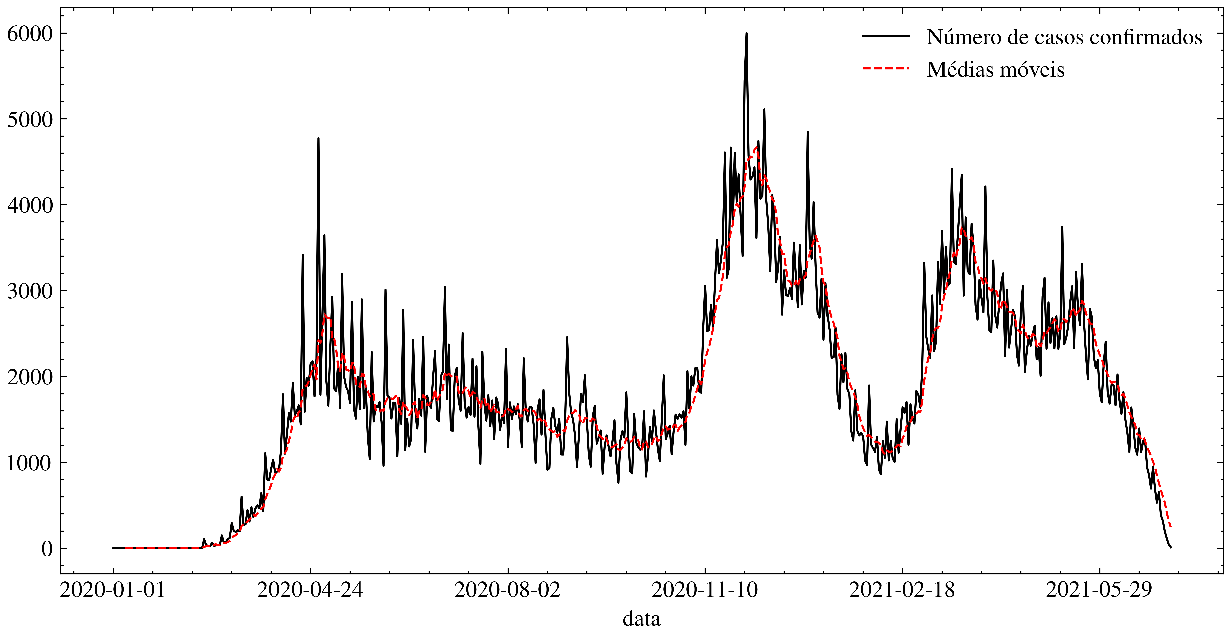
\includegraphics[width=5.0in]{img/casos_confirmados_ma.pdf}
    \caption{Médias móveis do número de casos confirmados de COVID-19 no Rio de Janeiro.}
    \label{fig:casos_confirmados_ma}
\end{figure}

\FloatBarrier

\subsection{Temperatura mínima diária em Melbourne}
Assim como na coleção de dados referente ao número de casos confirmados de COVID-19 no Rio de Janeiro~\ref{subsec:casos_confirmados}, os dados de temperatura mínima diária em Melbourne foram baixados através de um \textit{script} Python com o auxílio da biblioteca \textit{requests}. O arquivo pode ser baixado diretamente do GitHub \footnote{$https://raw.githubusercontent.com/jbrownlee/Datasets/master/daily-min-temperatures.csv$} e também pode ser encontrado em um desafio do Kaggle \footnote{$https://www.kaggle.com/paulbrabban/daily-minimum-temperatures-in-melbourne$}.

\begin{figure}[!htp]
    \centering
    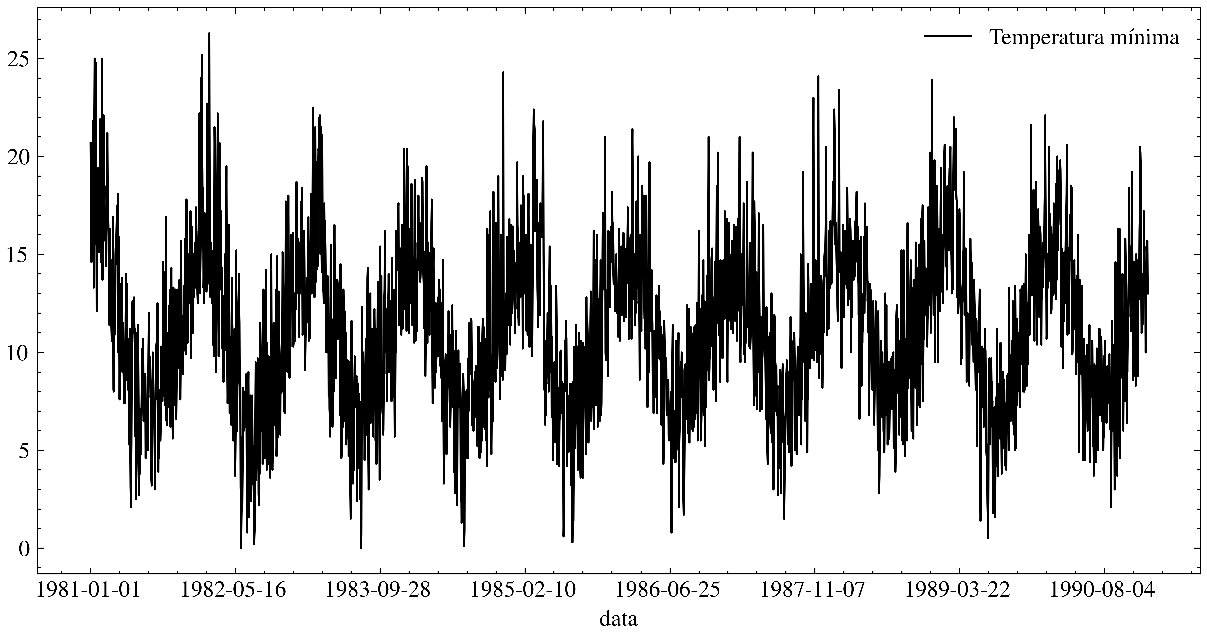
\includegraphics[width=5.0in]{img/temperatura_minima_diaria.pdf}
    \caption{Série temporal da temperatura mínima diária em Melbourne.}
    \label{fig:temperatura_minima_diaria}
\end{figure}

A Figura~\ref{fig:temperatura_minima_diaria} mostra que a quantidade de observações na série temporal da temperatura mínima diária em Melbourne é muito superior ao número de casos confirmados de COVID-19, e correspondem ao período entre 01/01/1981 e 31/12/1990. Outro ponto divergente é a observabilidade do caráter sazonal com período de um ano. Porém, as flutuações de curto prazo permanecem, e continuam configurando um problema para o ajuste de modelos preditivos que precisam generalizar para realizar inferências mais acertivas.

\begin{figure}[!htp]
    \centering
    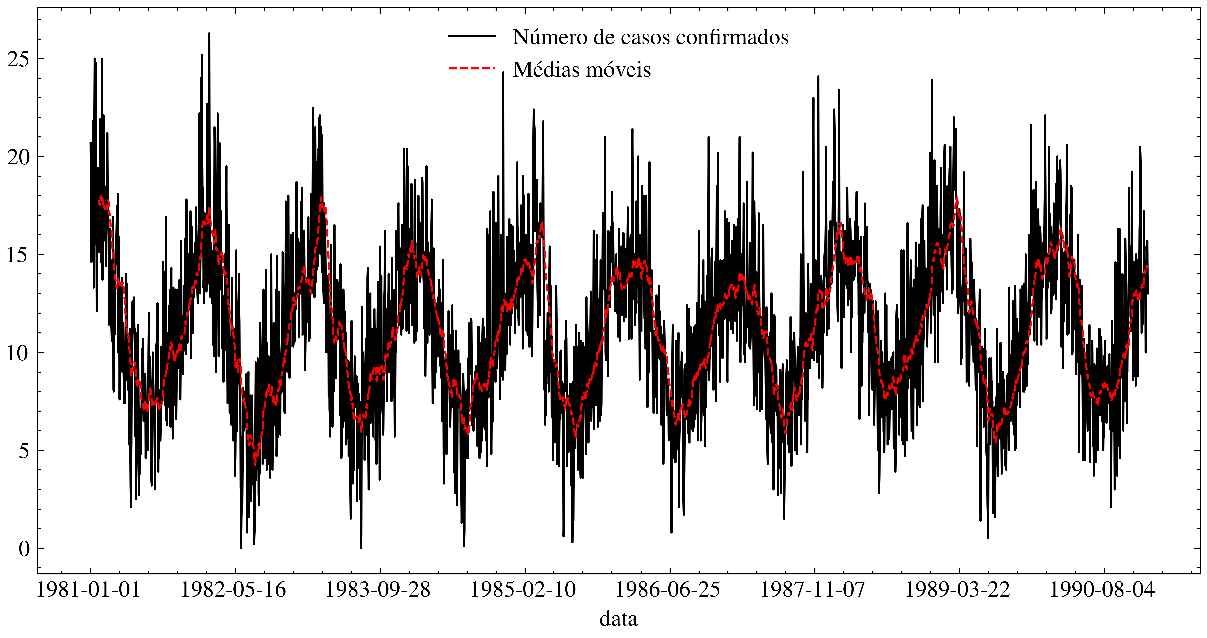
\includegraphics[width=5.0in]{img/temperatura_minima_diaria_ma.pdf}
    \caption{Médias móveis da temperatura mínima diária em Melbourne.}
    \label{fig:temperatura_minima_diaria_ma}
\end{figure}

A Figura~\ref{fig:temperatura_minima_diaria_ma} mostra as médias móveis da temperatura mínima diária em Melbourne em vermelho. O parâmetro utilizado para gerar esta figura foi $W=30$, que foi escolhido para representação gráfica por se tratar de uma série com aproximadamente um ano de período de sazonalidade.

\FloatBarrier

\subsection{Série temporal sintética}
Uma coleção de dados foi gerada de forma sintética com o auxílio da biblioteca \textit{numpy} do Python com características criadas artificialmente somando componentes como tendência, sazonalidade, ruído branco e fatores para distorção da estacionaridade seguindo o método apresentado em \citeauthor{syntheticdata}, \citeyear{syntheticdata} \cite{syntheticdata}. Essa série temporal é construída com o objetivo de avaliar a capacidade de generalização dos modelos em cima dos componentes que estes costumam considerar como base, justificando a importância de ter sido gerada sinteticamente.

Em uma série temporal, a tendência é o padrão que evidencia o crescimento ou decrescimento dos valores a longo prazo. Portanto, para compor a série temporal sintética, foi considerada uma função linear crescente como fator de tendência. A Figura~\ref{fig:upward_trend} mostra a componente resultante gerada sinteticamente.

\begin{figure}[!htp]
    \centering
    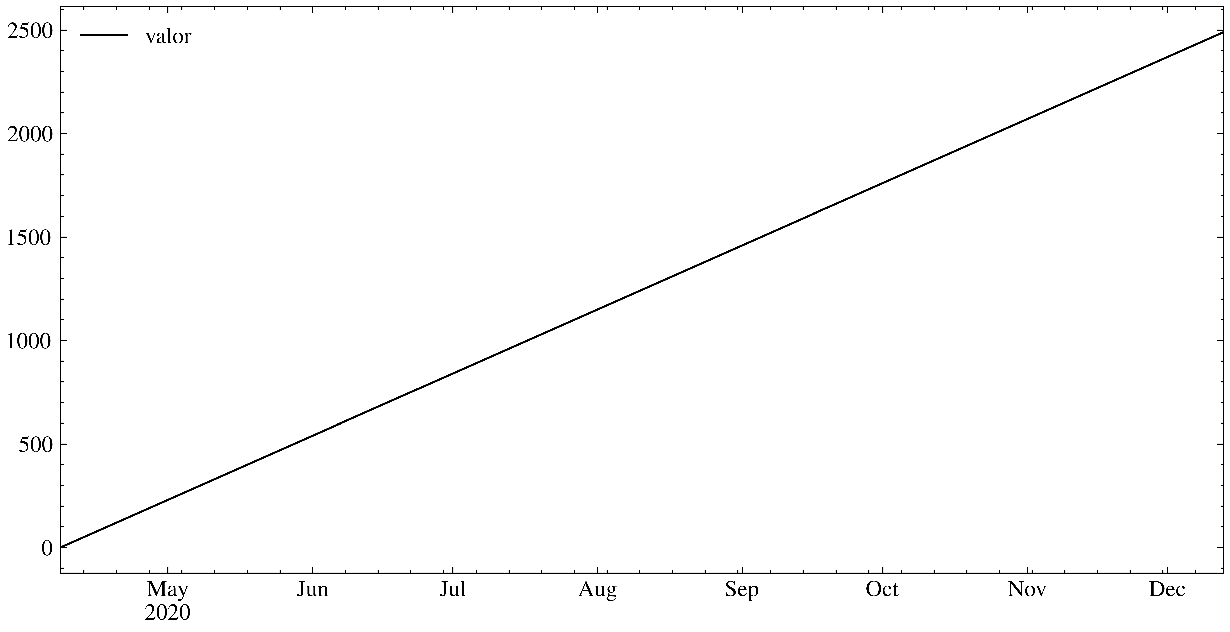
\includegraphics[width=5.0in]{img/upward_trend.pdf}
    \caption{Componente de tendência crescente.}
    \label{fig:upward_trend}
\end{figure}

A sasonalidade pode ser caracterizada pela presença de variações semelhantes que ocorrem em intervalos regulares de tempo. Então, para simular um comportamento sazonal, foi aplicado um crescimento cúbico seguido de um crescimento quadrático nos primeiros 50 dias, e então esse mesmo padrão foi repetido ao longo de toda a série temporal até o último dado observado. Na Figura~\ref{fig:seasonal_pattern} fica clara a repetição do padrão com as 2 curvas de crescimento seguidas.

\begin{figure}[!htp]
    \centering
    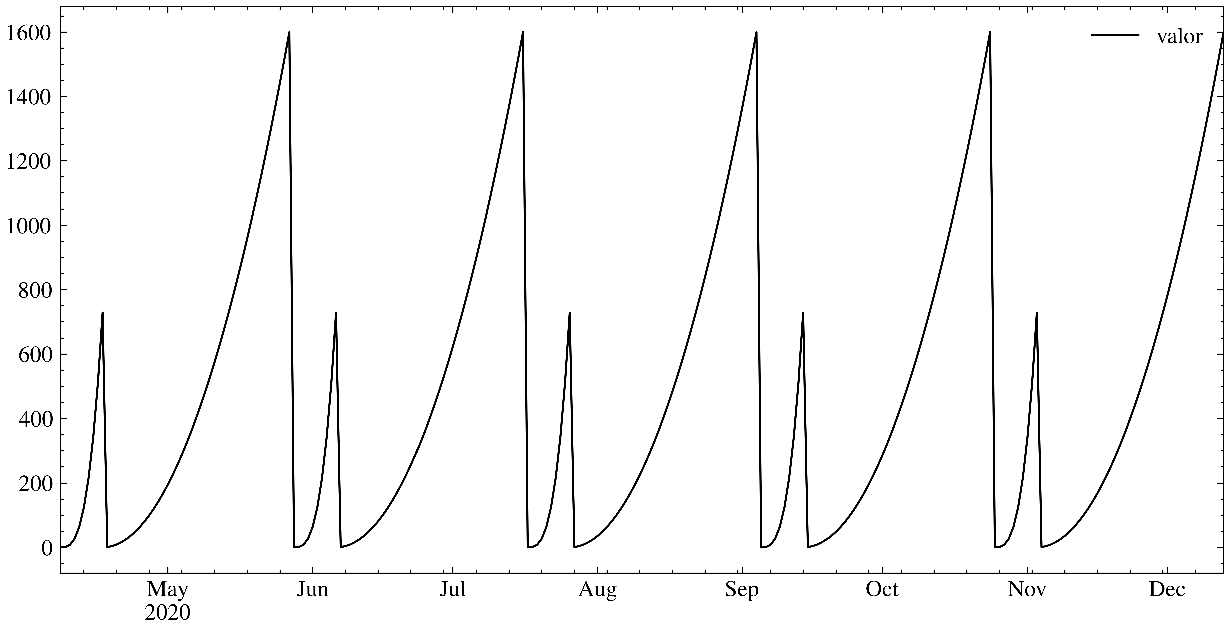
\includegraphics[width=5.0in]{img/seasonal_pattern.pdf}
    \caption{Componente de sazonalidade.}
    \label{fig:seasonal_pattern}
\end{figure}

O ruído é a parte do sinal que não possui valor semântico, ou seja, são distorções que ocorrem no sinal que podem ter como origem diversos fatores como o equipamento utilizado para fazer a coleta, erro humano, entre outros. Como nenhum sinal na vida real é livre de ruído, para aproximar a série temporal a de um problema real, foi adicionado um sinal de ruído branco gerado de forma pseudo-aleatória conforme apresentado na Figura~\ref{fig:noise}. Além do ruído, também foi adicionado um evento com impacto maior na série temporal com o objetivo de representar um fator inesperado na série. Esse fator pode ser equiparado a qualquer evento que possa alterar de forma disruptiva os dados observados na série temporal. Portanto, como a série possui uma tendência de crescimento, foi gerado um componente decrescente, ilustrado na Figura~\ref{fig:big_event}, nos últimos dias da série para ser somado aos outros componentes e gerar o efeito desejado.

\begin{figure}[!htp]
    \centering
    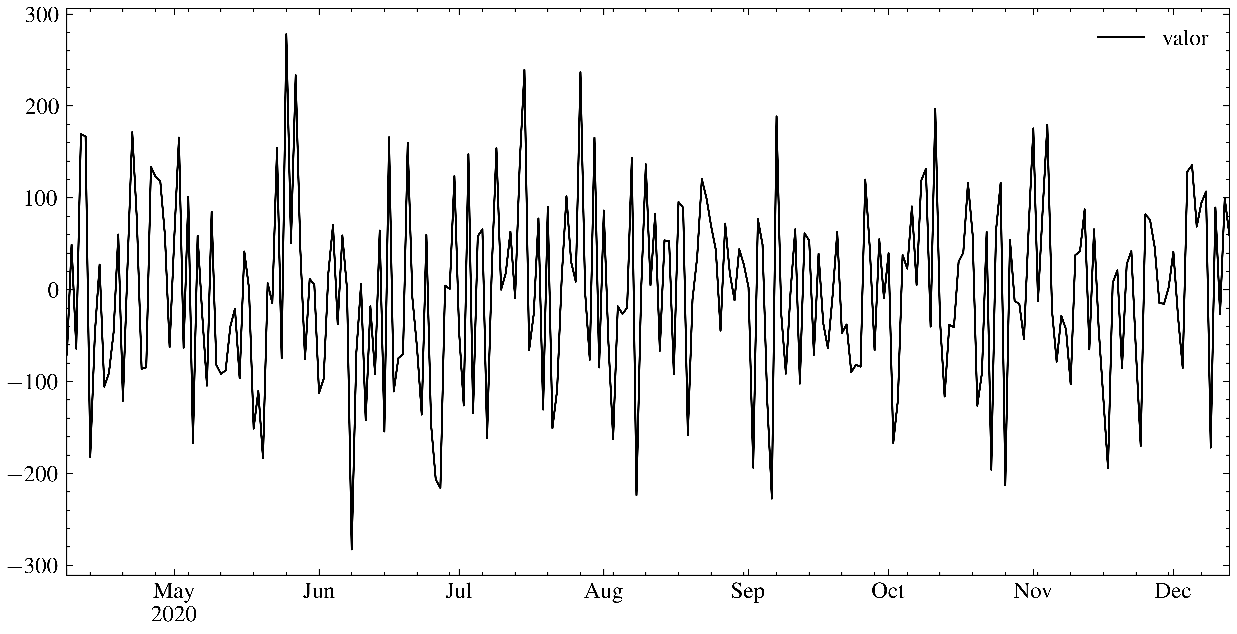
\includegraphics[width=5.0in]{img/noise.pdf}
    \caption{Ruído branco utilizado para compor a série temporal sintética.}
    \label{fig:noise}
\end{figure}

\begin{figure}[!htp]
    \centering
    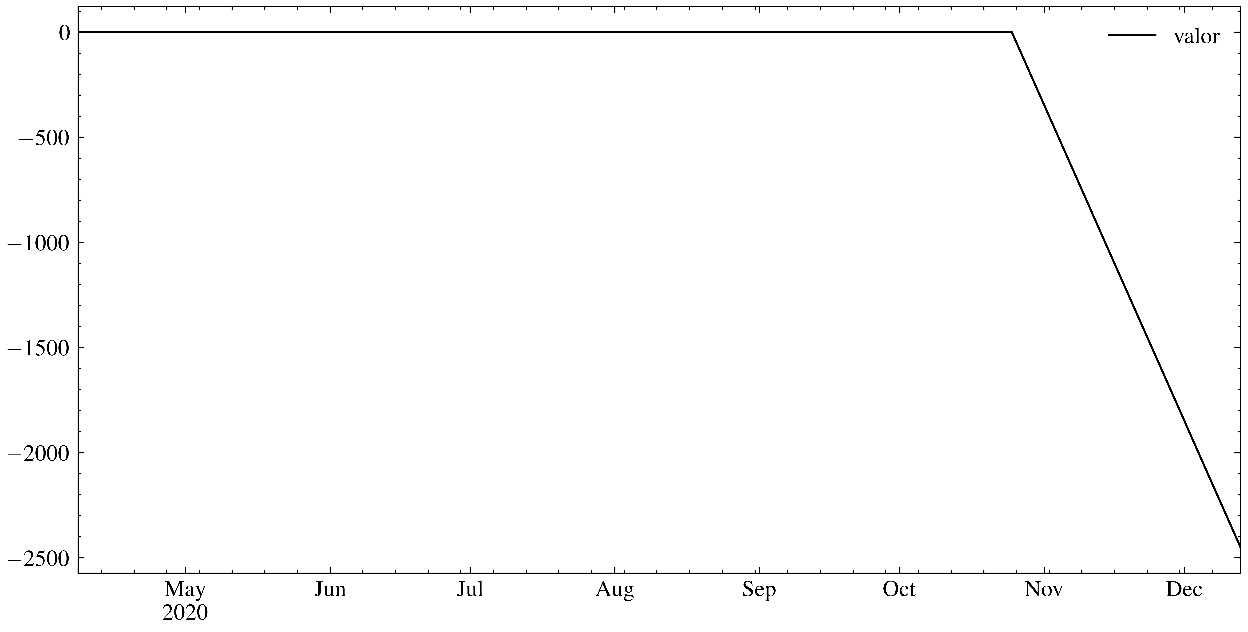
\includegraphics[width=5.0in]{img/big_event.pdf}
    \caption{Componente de evento inesperado descrescente.}
    \label{fig:big_event}
\end{figure}

Finalmente, após a soma de todos os componentes, é alcançada a série temporal resultante, conforme mostra a Figura~\ref{fig:dados_sinteticos}, onde será possível ajustar os modelos de predição e avaliar a capacidade de generalização de cada um. Como nas séries temporais anteriores, compartilha de flutuações de curto prazo, apesar de menores. Portanto, a Figura~\ref{fig:dados_sinteticos_ma} mostra as médias móveis calculadas com $W=4$ sobre a série temporal sintética. Esse valor foi escolhido na tentativa de suavizar as pequenas flutuações causadas propositalmente pela adição de ruído na composição da série temporal sintética.

\begin{figure}[!htp]
    \centering
    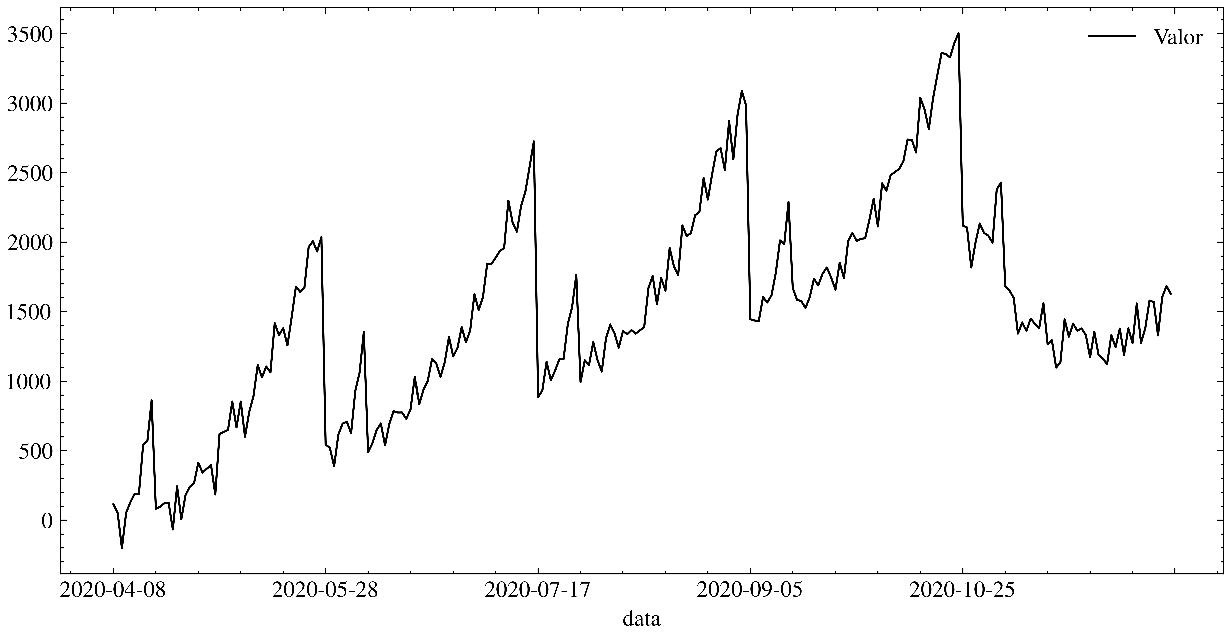
\includegraphics[width=5.0in]{img/dados_sinteticos.pdf}
    \caption{Série temporal gerada sinteticamente.}
    \label{fig:dados_sinteticos}
\end{figure}


\begin{figure}[!htp]
    \centering
    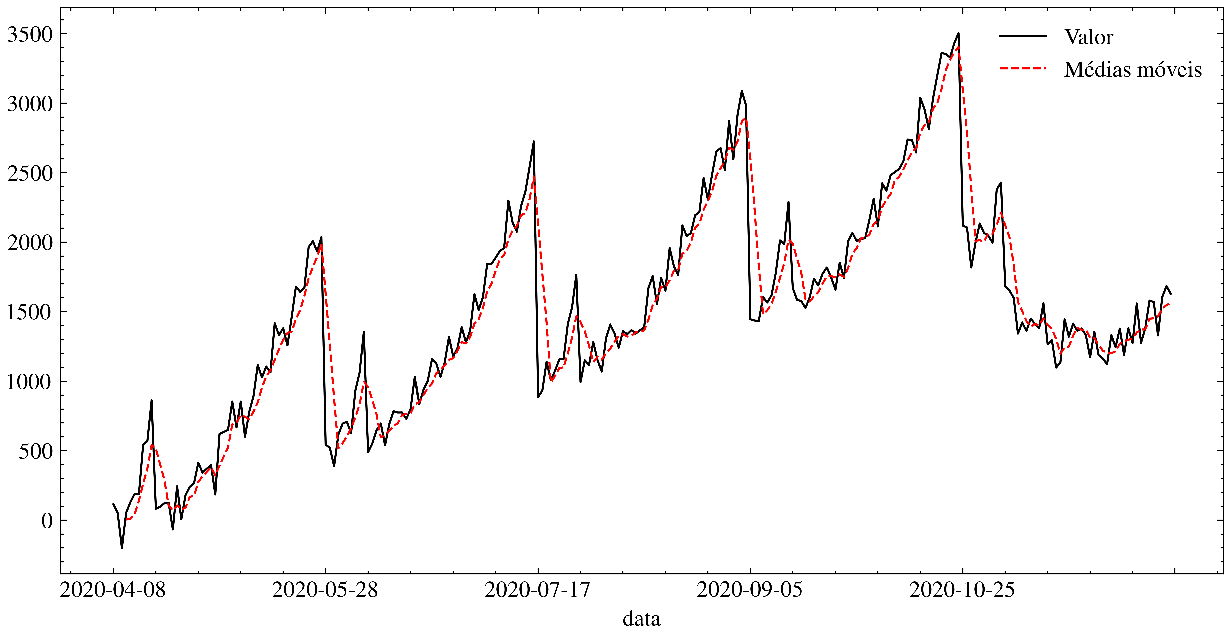
\includegraphics[width=5.0in]{img/dados_sinteticos_ma.pdf}
    \caption{Médias móveis da série temporal gerada sinteticamente.}
    \label{fig:dados_sinteticos_ma}
\end{figure}

\FloatBarrier

\section{Métricas de avaliação utilizadas} \label{sec:metrics}
Para a avaliação dos modelos preditivos, foram utilizadas 4 métricas de avaliação:  Raiz do Erro Médio Quadrático (\textit{Root Mean Square Error}, RMSE), \textit{Mean Absolute Error} (MAE), \textit{Mean Percentage Error} (MPE) e \textit{Mean Absolute Percentage Error} (MAPE). As métricas foram escolhidas com o objetivo de avaliar o erro de predição dos modelos de diferentes perspectivas. As Equações~\ref{eq:rmse}, \ref{eq:mae}, \ref{eq:mpe} e \ref{eq:mape} consideram $n$ como o número de observações presentes na coleção de dados, os valores de $y_{i}$ representam o conjunto de valores previstos pelos modelos e $x_{i}$ são os valores observados do conjunto separado para teste.

A Equação~\ref{eq:rmse} descreve o RMSE, que representa a raiz quadrada da média quadrática da diferença entre os valores previstos e observados. O RMSE é uma métrica que pode ser utilizada para comparar diferentes modelos ajustados e avaliados sobre um mesmo conjunto de dados, não sendo indicado para comparações entre coleções de dados diferentes. Esse comportamento é justificado pelo fato do RMSE ser uma métrica de acurácia que a escala depende da escala dos dados, como constatado em \cite{HYNDMAN2006679}. O valor de RMSE nunca assume valores negativos, e, em geral, valores menores são melhores que valores maiores. Esta métrica é sensível a erros muito grandes, ou seja, não possui um comportamento estável quando há \textit{outliers}.

\begin{equation} \label{eq:rmse}
    RMSE=\sqrt{\dfrac{\sum ^{n}_{i=1}\left( y_{i}-x_{i}\right) ^{2}}{n}}
\end{equation}

A métrica expressa pela Equação~\ref{eq:mae}, assim como o RMSE, é uma medida de acurácia. Com isso, compartilha da mesma propriedade de escala. A sua diferença principal, é que seu cálculo é linear, ou seja, as diferenças entre os valores observados e preditos são igualmente ponderadas na média.

\begin{equation} \label{eq:mae}
    MAE=\sum ^{n}_{i=1}\dfrac{\left| y_{i}-x_{i}\right| }{n}
\end{equation}

Diferente das métricas MAE, RMSE e MAPE, a \textit{Mean Percentage Error} (MPE), é uma métrica que considera o sinal do erro, ou seja, erros positivos e negativos se cancelam. Como consequência, a sua fórmula pode ser usada para medir o viés das predições. A Equação~\ref{eq:mpe} mostra como é feito o cáculo da MPE.

\begin{equation} \label{eq:mpe}
    MPE=\dfrac{1}{n}\sum ^{n}_{i=1}\dfrac{x_{i}-y_{i}}{x_{i}}
\end{equation}

A métrica \textit{Mean Absolute Percentage Error} (MAPE), é uma medida de acurácia, assim como a RMSE e MAE. Seu diferencial se dá pelo fato de ter uma interpretabilidade intuitiva comparado às outras métricas. Porém possui alguns defeitos bem conhecidos \cite{CHRISTOFALLIS2015}, como o erro da divisão por 0 e o fato de penalizar mais erros negativos do que erros positivos \cite{MAKRIDAKIS1993527}, levando à escolha de modelos cujo as predições são de valores mais baixos.

\begin{equation} \label{eq:mape}
    MAPE=\dfrac{1}{n}\sum ^{n}_{i=1}\left| \dfrac{y_{i}-x_{i}}{x_{i}}\right|
\end{equation}

\section{Resultados}
Os modelos Prophet, ARIMA e Regression WiSARD tiveram seus hiperparâmetros otimizados através de uma busca exaustiva em grade. Para cada modelo, foi definido um conjunto específico de combinações de hiperparâmetros que formaram um espaço discreto de busca, onde todas as possibilidades foram avaliadas. Os melhores conjuntos de hiperparâmetros encontrados para cada modelo, foram utilizados para uma comparação entre os modelos de acordo com 3 critérios: erro, tempo de inferência/ajuste e uso de memória RAM para inferência.

\subsection{Avaliação por métricas} \label{subsec:metrics_eval}
Para uma comparação quanto ao erro dos modelos, foram avaliadas as métricas explicadas na Seção~\ref{sec:metrics} para cada configuração possível da grade de hiperparâmetros de cada modelo. Cada modelo teve 4 configurações escolhidas, que foram otimizadas por cada uma das métricas apresentadas. As Tabelas~\ref{tab:temperature_results}, \ref{tab:covid_results} e \ref{tab:synthetic_results} mostram os resultados obtidos para cada \textit{dataset}.

\begin{table}[!htp]
    \caption{Tabela de métricas para o \textit{dataset} do número de casos confirmados de COVID-19 no Rio de Janeiro.}
    \label{tab:covid_results}
    \setlength\extrarowheight{5pt}
    \centering
    \begin{tabular}{|c|c|c|c|c|}
        \hline
        \rowcolor[HTML]{C0C0C0}
        Modelo  & RMSE                & MAPE              & MPE                & MAE                 \\ \hline
        ARIMA   & \textbf{238.181820} & \textbf{0.254128} & \textbf{-0.060560} & \textbf{194.656193} \\ \hline
        \rowcolor[HTML]{EFEFEF}
        rew     & 261.198655          & 5.029668          & -4.672775          & 226.856128          \\ \hline
        prophet & 1214.961631         & 21.895568         & -21.895568         & 1205.848658         \\ \hline
    \end{tabular}
\end{table}

\begin{table}[!htp]
    \caption{Tabela de métricas para o \textit{dataset} da temperatura mínima diária de Melbourne.}
    \label{tab:temperature_results}
    \setlength\extrarowheight{5pt}
    \centering
    \begin{tabular}{|c|c|c|c|c|}
        \hline
        \rowcolor[HTML]{C0C0C0}
        Modelo  & RMSE              & MAPE              & MPE                   & MAE               \\ \hline
        ARIMA   & 1.049886          & 0.060034          & -1.830924e-04         & 0.848392          \\ \hline
        \rowcolor[HTML]{EFEFEF}
        rew     & 0.910288          & \textbf{0.048378} & \textbf{5.457293e-08} & \textbf{0.700003} \\ \hline
        prophet & \textbf{0.905167} & 0.049002          & -1.334196e-04         & 0.707685          \\ \hline
    \end{tabular}
\end{table}

\begin{table}[!htp]
    \caption{Tabela de métricas para o \textit{dataset} gerado sinteticamente.}
    \label{tab:synthetic_results}
    \setlength\extrarowheight{5pt}
    \centering
    \begin{tabular}{|c|c|c|c|c|}
        \hline
        \rowcolor[HTML]{C0C0C0}
        Modelo  & RMSE                & MAPE              & MPE               & MAE                 \\ \hline
        ARIMA   & 131.741791          & 0.082449          & 0.006564          & 126.191932          \\ \hline
        \rowcolor[HTML]{EFEFEF}
        rew     & \textbf{126.377103} & \textbf{0.070265} & \textbf{0.000020} & \textbf{101.588470} \\ \hline
        prophet & 169.177431          & 0.100267          & 0.023560          & 153.021037          \\ \hline
    \end{tabular}
\end{table}


\subsection{Tempos de execução}
Para medir o tempo de execução, foram utilizados todos os melhores conjuntos de hiperparâmetros encontrados na busca de acordo com cada métrica, ou seja, foram realizados um total de 4 medições para cada modelo para cada \textit{dataset}. A medida de tempo do mesmo modelo com diferentes conjuntos de hiperparâmetros pode parecer irrelevante em um primeiro momento, mas pode indicar uma possível sensibilidade de performance dependendo do treinamento. A Tabela~\ref{tab:tempo_ajuste} mostra as medições de tempo feitas no momento da inferência, enquanto a Tabela~\ref{tab:tempo_inferencia} mostra as medições de tempo de inferência dos modelos. As medições de tempo de treinamento foram realizadas em 7 rodadas com 10 iterações, enquanto as de inferência foram obtidas com 7 rodadas de 100 iterações.

\begin{table}[!htp]
    \caption{Tempo de treinamento dos modelos.}
    \label{tab:tempo_ajuste}
    \setlength\extrarowheight{5pt}
    \begin{tabular}{|c|c|ccc|}
        \hline
        \rowcolor[HTML]{C0C0C0}
        \cellcolor[HTML]{C0C0C0}                          & \cellcolor[HTML]{C0C0C0}                          & \multicolumn{3}{c|}{\cellcolor[HTML]{C0C0C0}Dataset}                                                                                                                         \\ \cline{3-5}
        \rowcolor[HTML]{C0C0C0}
        \multirow{-2}{*}{\cellcolor[HTML]{C0C0C0}Modelo}  & \multirow{-2}{*}{\cellcolor[HTML]{C0C0C0}Métrica} & \multicolumn{1}{c|}{\cellcolor[HTML]{C0C0C0}COVID}                      & \multicolumn{1}{c|}{\cellcolor[HTML]{C0C0C0}Temperatura}               & Sintético                 \\ \hline
        \cellcolor[HTML]{C0C0C0}                          & RMSE                                              & \multicolumn{1}{c|}{779 ms ± 2.4 ms}                                    & \multicolumn{1}{c|}{3.61 s ± 5.34 ms}                                  & 38.4 ms ± 383 µs          \\ \cline{2-5}
        \rowcolor[HTML]{EFEFEF}
        \cellcolor[HTML]{C0C0C0}                          & MAPE                                              & \multicolumn{1}{c|}{\cellcolor[HTML]{EFEFEF}1.34 s ± 2.11ms}            & \multicolumn{1}{c|}{\cellcolor[HTML]{EFEFEF}3.61 s ± 4.68 ms}          & 38.3 ms ± 184 µs          \\ \cline{2-5}
        \cellcolor[HTML]{C0C0C0}                          & MAE                                               & \multicolumn{1}{c|}{779 ms ± 1.2 ms}                                    & \multicolumn{1}{c|}{3.61 s ± 8.5 ms}                                   & 38.4 ms ± 225 µs          \\ \cline{2-5}
        \rowcolor[HTML]{EFEFEF}
        \multirow{-4}{*}{\cellcolor[HTML]{C0C0C0}ARIMA}   & MPE                                               & \multicolumn{1}{c|}{\cellcolor[HTML]{EFEFEF}1.61 s ± 1.33 ms}           & \multicolumn{1}{c|}{\cellcolor[HTML]{EFEFEF}6.36 s ± 9.48 ms}          & 566 ms ± 705 µs           \\ \hline
        \cellcolor[HTML]{C0C0C0}                          & RMSE                                              & \multicolumn{1}{c|}{\textbf{4.41 ms ± 151 µs}}                          & \multicolumn{1}{c|}{\textbf{31.2 ms ± 526 µs}}                         & \textbf{9.97 ms ± 143 µs} \\ \cline{2-5}
        \rowcolor[HTML]{EFEFEF}
        \cellcolor[HTML]{C0C0C0}                          & MAPE                                              & \multicolumn{1}{c|}{\cellcolor[HTML]{EFEFEF}\textbf{4.46 ms ± 75.1 µs}} & \multicolumn{1}{c|}{\cellcolor[HTML]{EFEFEF}\textbf{19.5 ms ± 409 µs}} & \textbf{10.1 ms ± 166 µs} \\ \cline{2-5}
        \cellcolor[HTML]{C0C0C0}                          & MAE                                               & \multicolumn{1}{c|}{\textbf{8.65 ms ± 126 µs}}                          & \multicolumn{1}{c|}{\textbf{19.3 ms ± 149 µs}}                         & \textbf{10.5 ms ± 116 µs} \\ \cline{2-5}
        \rowcolor[HTML]{EFEFEF}
        \multirow{-4}{*}{\cellcolor[HTML]{C0C0C0}ReW}     & MPE                                               & \multicolumn{1}{c|}{\cellcolor[HTML]{EFEFEF}\textbf{4.41 ms ± 151 µs}}  & \multicolumn{1}{c|}{\cellcolor[HTML]{EFEFEF}\textbf{64.7 ms ± 549 µs}} & \textbf{8.86 ms ± 123 µs} \\ \hline
        \cellcolor[HTML]{C0C0C0}                          & RMSE                                              & \multicolumn{1}{c|}{56.5 ms ± 17.9 ms}                                  & \multicolumn{1}{c|}{205 ms ± 176 µs}                                   & 60.7 ms ± 87 µs           \\ \cline{2-5}
        \rowcolor[HTML]{EFEFEF}
        \cellcolor[HTML]{C0C0C0}                          & MAPE                                              & \multicolumn{1}{c|}{\cellcolor[HTML]{EFEFEF}46 ms ± 63.1 µs}            & \multicolumn{1}{c|}{\cellcolor[HTML]{EFEFEF}179 ms ± 514 µs}           & 60.9 ms ± 174 µs          \\ \cline{2-5}
        \cellcolor[HTML]{C0C0C0}                          & MAE                                               & \multicolumn{1}{c|}{44.6 ms ± 109 µs}                                   & \multicolumn{1}{c|}{180 ms ± 396 µs}                                   & 61.1 ms ± 177 µs          \\ \cline{2-5}
        \rowcolor[HTML]{EFEFEF}
        \multirow{-4}{*}{\cellcolor[HTML]{C0C0C0}Prophet} & MPE                                               & \multicolumn{1}{c|}{\cellcolor[HTML]{EFEFEF}46 ms ± 72.1 µs}            & \multicolumn{1}{c|}{\cellcolor[HTML]{EFEFEF}203 ms ± 200 µs}           & 68.1 ms ± 178 µs          \\ \hline
    \end{tabular}
\end{table}

\begin{table}[!htp]
    \caption{Tempo de inferência dos modelos.}
    \label{tab:tempo_inferencia}
    \setlength\extrarowheight{5pt}
    \begin{tabular}{|c|c|ccc|}
        \hline
        \rowcolor[HTML]{C0C0C0}
        \cellcolor[HTML]{C0C0C0}                          & \cellcolor[HTML]{C0C0C0}                          & \multicolumn{3}{c|}{\cellcolor[HTML]{C0C0C0}Dataset}                                                                                                                         \\ \cline{3-5}
        \rowcolor[HTML]{C0C0C0}
        \multirow{-2}{*}{\cellcolor[HTML]{C0C0C0}Modelo}  & \multirow{-2}{*}{\cellcolor[HTML]{C0C0C0}Métrica} & \multicolumn{1}{c|}{\cellcolor[HTML]{C0C0C0}COVID}                      & \multicolumn{1}{c|}{\cellcolor[HTML]{C0C0C0}Temperatura}               & Sintético                 \\ \hline
        \cellcolor[HTML]{C0C0C0}                          & RMSE                                              & \multicolumn{1}{c|}{960 µs ± 2.51 µs}                                   & \multicolumn{1}{c|}{951 µs ± 14.4 µs}                                  & 1.92 ms ± 28.5 µs         \\ \cline{2-5}
        \rowcolor[HTML]{EFEFEF}
        \cellcolor[HTML]{C0C0C0}                          & MAPE                                              & \multicolumn{1}{c|}{\cellcolor[HTML]{EFEFEF}970 µs ± 1.83 µs}           & \multicolumn{1}{c|}{\cellcolor[HTML]{EFEFEF}942 µs ± 4.96 µs}          & 1.93 ms ± 33.3 µs         \\ \cline{2-5}
        \cellcolor[HTML]{C0C0C0}                          & MAE                                               & \multicolumn{1}{c|}{958 µs ± 2.81 µs}                                   & \multicolumn{1}{c|}{972 µs ± 8.09 µs}                                  & 1.92 ms ± 24.8 µs         \\ \cline{2-5}
        \rowcolor[HTML]{EFEFEF}
        \multirow{-4}{*}{\cellcolor[HTML]{C0C0C0}ARIMA}   & MPE                                               & \multicolumn{1}{c|}{\cellcolor[HTML]{EFEFEF}959 µs ± 5.72 µs}           & \multicolumn{1}{c|}{\cellcolor[HTML]{EFEFEF}956 µs ± 7.02 µs}          & 953 µs ± 27.8 µs          \\ \hline
        \cellcolor[HTML]{C0C0C0}                          & RMSE                                              & \multicolumn{1}{c|}{\textbf{142 µs ± 2.8 µs}}                           & \multicolumn{1}{c|}{\textbf{149 µs ± 349 ns}}                          & \textbf{330 µs ± 4.67}    \\ \cline{2-5}
        \rowcolor[HTML]{EFEFEF}
        \cellcolor[HTML]{C0C0C0}                          & MAPE                                              & \multicolumn{1}{c|}{\cellcolor[HTML]{EFEFEF}\textbf{87.6 µs ± 1.22 µs}} & \multicolumn{1}{c|}{\cellcolor[HTML]{EFEFEF}\textbf{106 µs ± 339 ns}}  & \textbf{494 µs ± 12.8 µs} \\ \cline{2-5}
        \cellcolor[HTML]{C0C0C0}                          & MAE                                               & \multicolumn{1}{c|}{\textbf{145 µs ± 2.3 µs}}                           & \multicolumn{1}{c|}{\textbf{107 µs ± 1.45 µs}}                         & \textbf{512 µs ± 7.91 µs} \\ \cline{2-5}
        \rowcolor[HTML]{EFEFEF}
        \multirow{-4}{*}{\cellcolor[HTML]{C0C0C0}ReW}     & MPE                                               & \multicolumn{1}{c|}{\cellcolor[HTML]{EFEFEF}\textbf{91 µs ± 638 ns}}    & \multicolumn{1}{c|}{\cellcolor[HTML]{EFEFEF}\textbf{232 µs ± 6.43 µs}} & \textbf{422 µs ± 8.16 µs} \\ \hline
        \cellcolor[HTML]{C0C0C0}                          & RMSE                                              & \multicolumn{1}{c|}{1.26 s ± 10.7 ms}                                   & \multicolumn{1}{c|}{1.88 s ± 3.79 ms}                                  & 898 ms ± 768 µs           \\ \cline{2-5}
        \rowcolor[HTML]{EFEFEF}
        \cellcolor[HTML]{C0C0C0}                          & MAPE                                              & \multicolumn{1}{c|}{\cellcolor[HTML]{EFEFEF}1.25 s ± 1.59 ms}           & \multicolumn{1}{c|}{\cellcolor[HTML]{EFEFEF}2.13 s ± 711 µs}           & 906 ms ± 600 µs           \\ \cline{2-5}
        \cellcolor[HTML]{C0C0C0}                          & MAE                                               & \multicolumn{1}{c|}{1.25 s ± 1.29 ms}                                   & \multicolumn{1}{c|}{2.13 s ± 940 µs}                                   & 898 ms ± 753 µs           \\ \cline{2-5}
        \rowcolor[HTML]{EFEFEF}
        \multirow{-4}{*}{\cellcolor[HTML]{C0C0C0}Prophet} & MPE                                               & \multicolumn{1}{c|}{\cellcolor[HTML]{EFEFEF}1.25 s ± 1.26 ms}           & \multicolumn{1}{c|}{\cellcolor[HTML]{EFEFEF}1.88 s ± 530 µs}           & 899 ms ± 1.24 ms          \\ \hline
    \end{tabular}
\end{table}

\FloatBarrier

\subsection{Uso de memória}
Assim como as medidas de tempo de execução, o uso de memória foi coletado para cada combinação de modelo, \textit{dataset} e métrica utilizada para escolha dos hiperparâmetros. Porém, neste caso, a medida de interesse é o uso de memória do modelo ajustado, portanto a Tabela~\ref{tab:memoria} mostra o uso de memória em MiB de cada modelo. As medidas foram realizadas com o auxílio da biblioteca \textit{memory\_profiler}, que possui todas suas especificações documentadas no github\footnote{$https://github.com/pythonprofilers/memory\_profiler\#memory-profiler$}.


\begin{table}[!htp]
    \caption{Uso de memória de cada modelo por métrica otimizada e dataset.}
    \label{tab:memoria}
    \setlength\extrarowheight{5pt}
    \centering
    \begin{tabular}{|c|c|ccc|}
        \hline
        \rowcolor[HTML]{C0C0C0}
        \cellcolor[HTML]{C0C0C0}                          & \cellcolor[HTML]{C0C0C0}                          & \multicolumn{3}{c|}{\cellcolor[HTML]{C0C0C0}Dataset}                                                                                                   \\ \cline{3-5}
        \rowcolor[HTML]{C0C0C0}
        \multirow{-2}{*}{\cellcolor[HTML]{C0C0C0}Modelo}  & \multirow{-2}{*}{\cellcolor[HTML]{C0C0C0}Métrica} & \multicolumn{1}{c|}{\cellcolor[HTML]{C0C0C0}COVID}              & \multicolumn{1}{c|}{\cellcolor[HTML]{C0C0C0}Temperatura}        & Sintético          \\ \hline
        \cellcolor[HTML]{C0C0C0}                          & RMSE                                              & \multicolumn{1}{c|}{9.086 MiB}                                  & \multicolumn{1}{c|}{43.621 MiB}                                 & 3.105 MiB          \\ \cline{2-5}
        \rowcolor[HTML]{EFEFEF}
        \cellcolor[HTML]{C0C0C0}                          & MAPE                                              & \multicolumn{1}{c|}{\cellcolor[HTML]{EFEFEF}11.383 MiB}         & \multicolumn{1}{c|}{\cellcolor[HTML]{EFEFEF}43.699 MiB}         & 3.078 MiB          \\ \cline{2-5}
        \cellcolor[HTML]{C0C0C0}                          & MAE                                               & \multicolumn{1}{c|}{8.816 MiB}                                  & \multicolumn{1}{c|}{44.035 MiB}                                 & 3.359 MiB          \\ \cline{2-5}
        \rowcolor[HTML]{EFEFEF}
        \multirow{-4}{*}{\cellcolor[HTML]{C0C0C0}ARIMA}   & MPE                                               & \multicolumn{1}{c|}{\cellcolor[HTML]{EFEFEF}13.734 MiB}         & \multicolumn{1}{c|}{\cellcolor[HTML]{EFEFEF}50.805 MiB}         & 6.457 MiB          \\ \hline
        \cellcolor[HTML]{C0C0C0}                          & RMSE                                              & \multicolumn{1}{c|}{\textbf{0.512 MiB}}                         & \multicolumn{1}{c|}{\textbf{1.039 MiB}}                         & \textbf{0.598 MiB} \\ \cline{2-5}
        \rowcolor[HTML]{EFEFEF}
        \cellcolor[HTML]{C0C0C0}                          & MAPE                                              & \multicolumn{1}{c|}{\cellcolor[HTML]{EFEFEF}\textbf{0.000 MiB}} & \multicolumn{1}{c|}{\cellcolor[HTML]{EFEFEF}\textbf{0.922 MiB}} & \textbf{0.570 MiB} \\ \cline{2-5}
        \cellcolor[HTML]{C0C0C0}                          & MAE                                               & \multicolumn{1}{c|}{\textbf{0.586 MiB}}                         & \multicolumn{1}{c|}{\textbf{0.887 MiB}}                         & \textbf{0.898 MiB} \\ \cline{2-5}
        \rowcolor[HTML]{EFEFEF}
        \multirow{-4}{*}{\cellcolor[HTML]{C0C0C0}ReW}     & MPE                                               & \multicolumn{1}{c|}{\cellcolor[HTML]{EFEFEF}\textbf{0.645 MiB}} & \multicolumn{1}{c|}{\cellcolor[HTML]{EFEFEF}\textbf{0.809 MiB}} & \textbf{0.562 MiB} \\ \hline
        \cellcolor[HTML]{C0C0C0}                          & RMSE                                              & \multicolumn{1}{c|}{90.676 MiB}                                 & \multicolumn{1}{c|}{101.699 MiB}                                & 89.719 MiB         \\ \cline{2-5}
        \rowcolor[HTML]{EFEFEF}
        \cellcolor[HTML]{C0C0C0}                          & MAPE                                              & \multicolumn{1}{c|}{\cellcolor[HTML]{EFEFEF}90.652 MiB}         & \multicolumn{1}{c|}{\cellcolor[HTML]{EFEFEF}102.074 MiB}        & 89.203 MiB         \\ \cline{2-5}
        \cellcolor[HTML]{C0C0C0}                          & MAE                                               & \multicolumn{1}{c|}{90.621 MiB}                                 & \multicolumn{1}{c|}{102.273 MiB}                                & 89.426 MiB         \\ \cline{2-5}
        \rowcolor[HTML]{EFEFEF}
        \multirow{-4}{*}{\cellcolor[HTML]{C0C0C0}Prophet} & MPE                                               & \multicolumn{1}{c|}{\cellcolor[HTML]{EFEFEF}90.617 MiB}         & \multicolumn{1}{c|}{\cellcolor[HTML]{EFEFEF}101.926 MiB}        & 89.277 MiB         \\ \hline
    \end{tabular}
\end{table}

\FloatBarrier

\subsection{Discussão}
Com base nos resultados expostos na Subseção~\ref{subsec:metrics_eval}, é possível concluir que todos os modelos atingiram métricas próximas considerando suas respectivas escalas. Na maioria dos casos, todas as métricas apontaram o mesmo modelo como melhor opção, tendo como exceção apenas o \textit{dataset} de temperatura mínima diária em Melbourne, que teve o modelo Prophet apontado como melhor opção ao considerar a métrica RMSE. Ao observar as Tabelas~\ref{tab:temperature_results} e \ref{tab:synthetic_results}, é possível também notar a propriedade das métricas dependentes da escala, conforme descrito na Subseção~\ref{subsec:metrics_eval}. Em geral, a Regression WiSARD obteve a melhor performance para as coleções de dados sintética e temperatura mínima diária em Melbourne, enquanto o ARIMA obeteve o melhor resultado para o número de casos confirmados de COVID-19 no Rio de Janeiro.

Os resultados referentes ao tempo de treinamento, por sua vez, favoreceram o modelo Regression WiSARD, apresentando tempos de treinamento ordens de grandeza menores que o ARIMA e o Prophet. Apesar disto, o Prophet apresentou um tempo de treinamento significativamente menor se comparado ao ARIMA. O tempo de inferência também privilegiou a Regression WiSARD, porém o modelo ARIMA obteve tempos significativamente melhores que o Prophet, se mantendo, em alguns casos, quase na mesma ordem de grandeza dos tempos da Regression WiSARD. O tamanho do \textit{dataset} foi uma característica relevante para o tempo de treinamento, dado que houve aumento no tempo medido em \textit{datasets} maiores.

Em relação ao uso de memória RAM, a Regression WiSARD apresentou o menor custo, seguida do ARIMA e do Prophet, respectivamente. Independente do \textit{dataset} e do conjunto de hiperparâmetros utilizado, houve unanimidade na comparação de uso de memória entre os 3 modelos, porém, o ARIMA foi o modelo que mais sofreu variações com o tamanho do \textit{dataset}, apesar de sempre se manter com uso de memória inferior ao Prophet.
\chapter{Conclusão}
\label{chap:06}

Este trabalho começou apresentando dois modelos de previsão de séries temporais e descrevendo suas características e implementações. Então, foi apresentado um modelo de regressão supervisionado baseado em Redes Neurais sem Peso e um método alternativo para resolver o problema de previsão de séries temporais. A transformação do problema de previsão de séries temporais em um problema de regressão supervisionado através das janelas deslizantes e a suavização das flutuações de curto prazo com médias móveis foram essenciais para viabilizar o treinamento do modelo avaliado.

O método apresentado provou ser competitivo nas medidas de acurácia em relação a modelos como o ARIMA e o Prophet na resolução do problema de previsão do número de casos confirmados de COVID-19 no Rio de Janeiro, da temperatura mínima diária em Melbourne e de dados gerados de forma sintética. Em relação ao tempo de inferência e ajuste o modelo utilizado foi superior aos demais modelos, assim como na utilização de memória. Portanto, dado a baixa utilização de memória e o baixo tempo de inferência e ajuste, este método é um bom candidato para situações onde o custo computacional seja um requisito relevante.

Apesar de terem sido obtidos resultados satisfatórios no método apresentado, a utilização de comitês pode ser explorada como trabalho futuro em curto prazo, além da possibilidade de realizar predições de multiplos passos à frente, que podem melhorar a acurácia do modelo mantendo o baixo custo computacional. A utilização de variáveis exógenas também pode ser explorada, porém requer pouco mais tempo para o estudo de como incluir estas no treinamento de forma que melhore os resultados. Já a longo prazo, podem ser pensadas formas de previsões de séries temporais com múltiplas variáveis de saída e em técnicas de pré-processamento para séries temporais de alta frequência como uma tentativa de melhoria em relação a acurácia, sem que haja perda significativa no custo computacional.


\backmatter
\bibliographystyle{coppe-unsrt}
\bibliography{main}

\appendix
\chapter{Comparação das métricas por modelo e conjunto de dados}
\label{apen:a}

Para a comparação das métricas de erro entre os modelos utilizados nos experimentos, foram utilizados gráficos de barras. O eixo das ordenadas é composto pela métrica de erro utilizada na comparação, enquanto o eixo das abscissas contém o identificador das barras, que são os modelos. Para manter a coerência, o modelo ARIMA foi sempre representado pela cor preta, enquanto o Prophet pela cor vermelha e a ReW pela azul.

\begin{figure}[!htp]
    \centering
    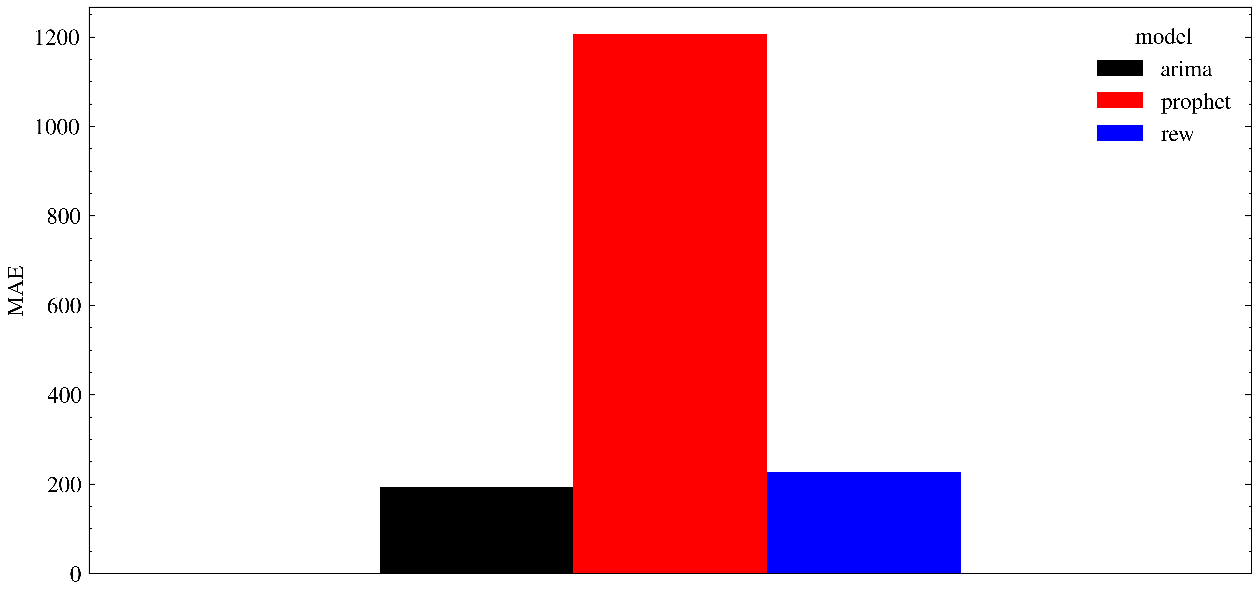
\includegraphics[width=5.0in]{img/covid_mae_comparison.pdf}
    \caption{MAE por modelo para o número de casos confirmados de COVID-19.}
\end{figure}

\begin{figure}[!htp]
    \centering
    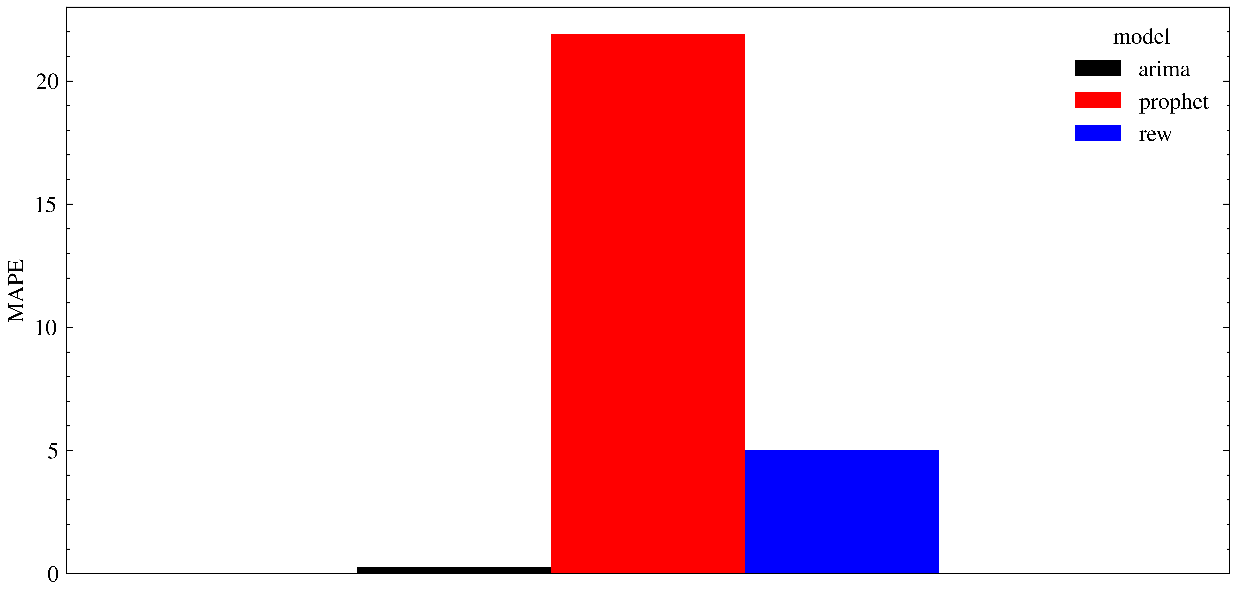
\includegraphics[width=5.0in]{img/covid_mape_comparison.pdf}
    \caption{MAPE por modelo para o número de casos confirmados de COVID-19.}
\end{figure}

\begin{figure}[!htp]
    \centering
    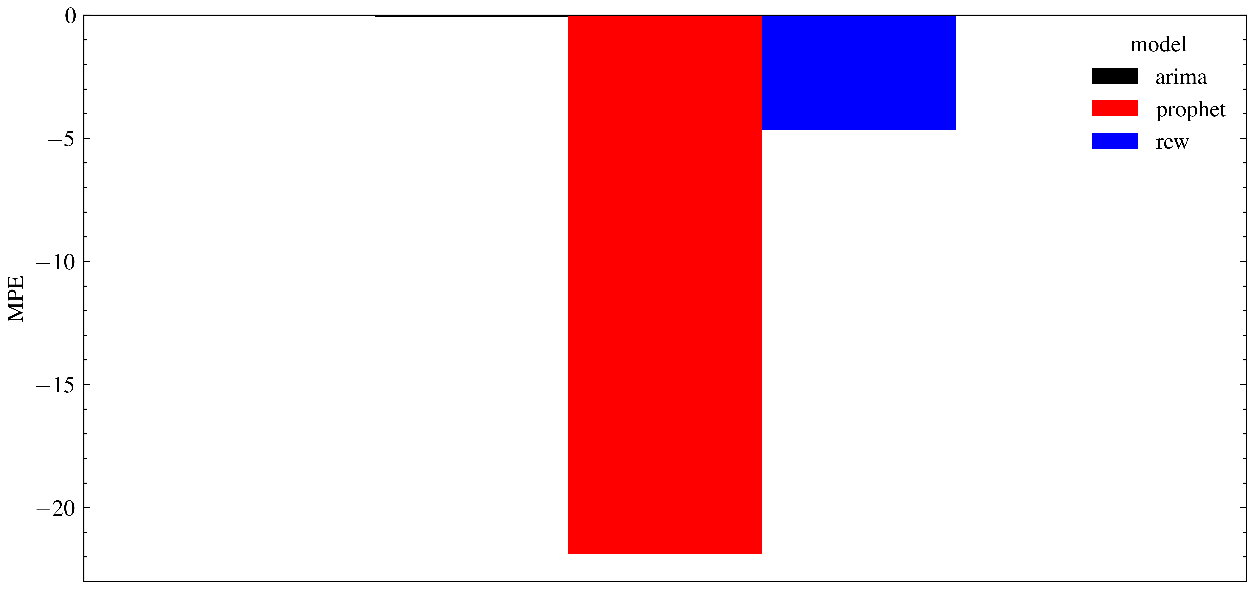
\includegraphics[width=5.0in]{img/covid_mpe_comparison.pdf}
    \caption{MPE por modelo para o número de casos confirmados de COVID-19.}
\end{figure}

\begin{figure}[!htp]
    \centering
    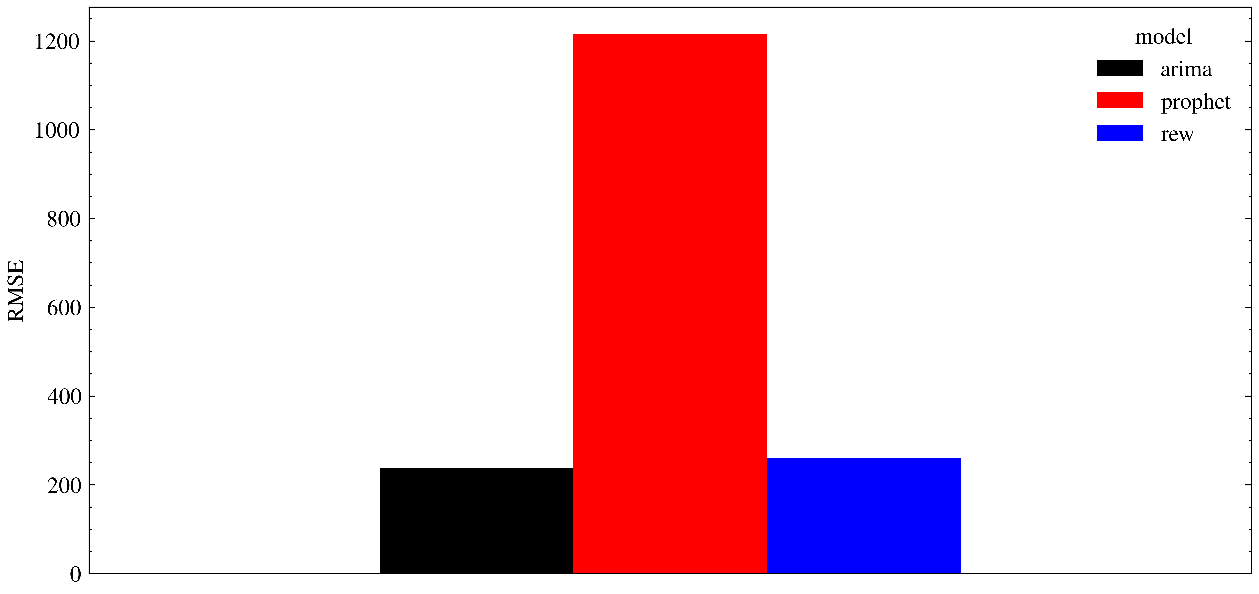
\includegraphics[width=5.0in]{img/covid_rmse_comparison.pdf}
    \caption{RMSE por modelo para o número de casos confirmados de COVID-19.}
\end{figure}

\begin{figure}[!htp]
    \centering
    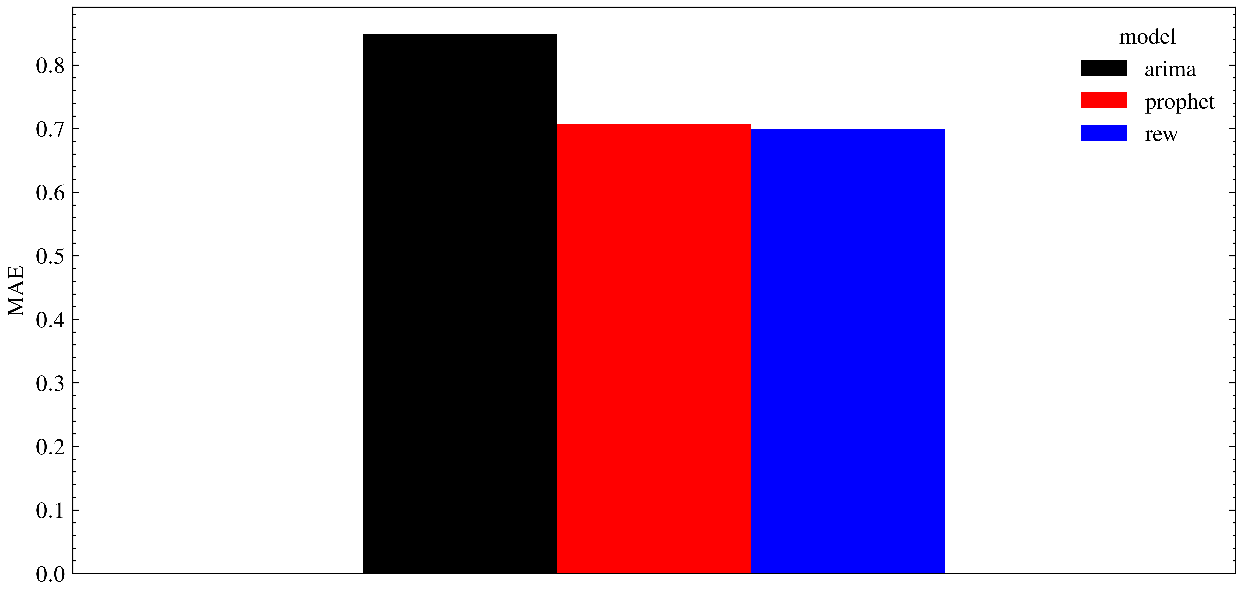
\includegraphics[width=5.0in]{img/temperatures_mae_comparison.pdf}
    \caption{MAE por modelo para a temperatura diária de Melbourne.}
\end{figure}

\begin{figure}[!htp]
    \centering
    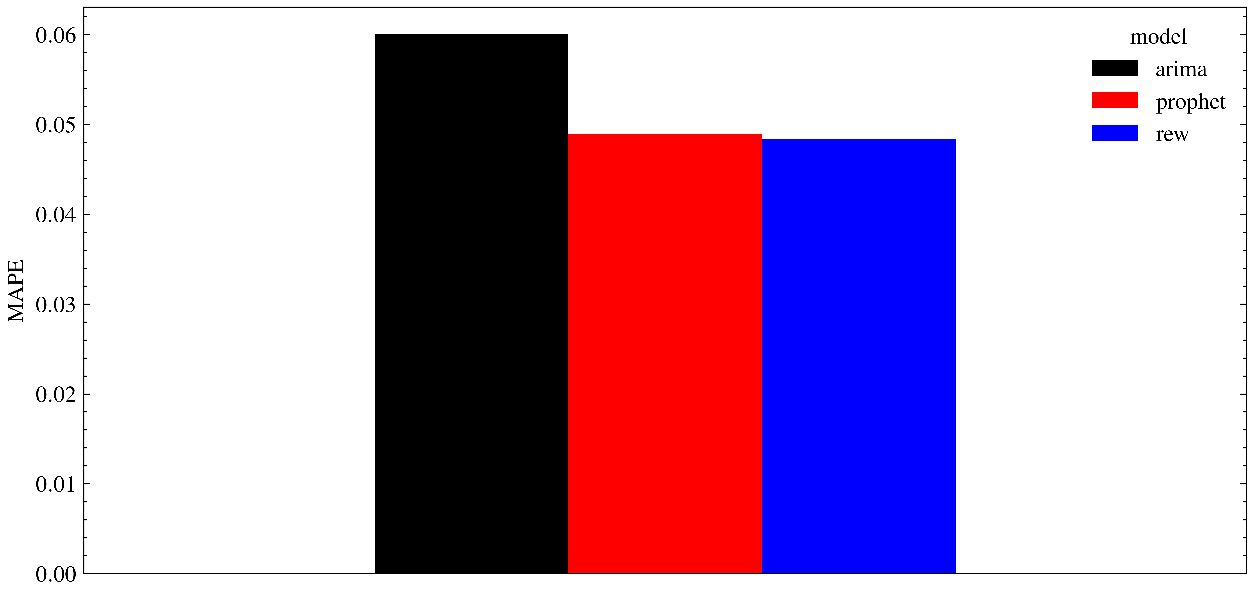
\includegraphics[width=5.0in]{img/temperatures_mape_comparison.pdf}
    \caption{MAPE por modelo para a temperatura diária de Melbourne}
\end{figure}

\begin{figure}[!htp]
    \centering
    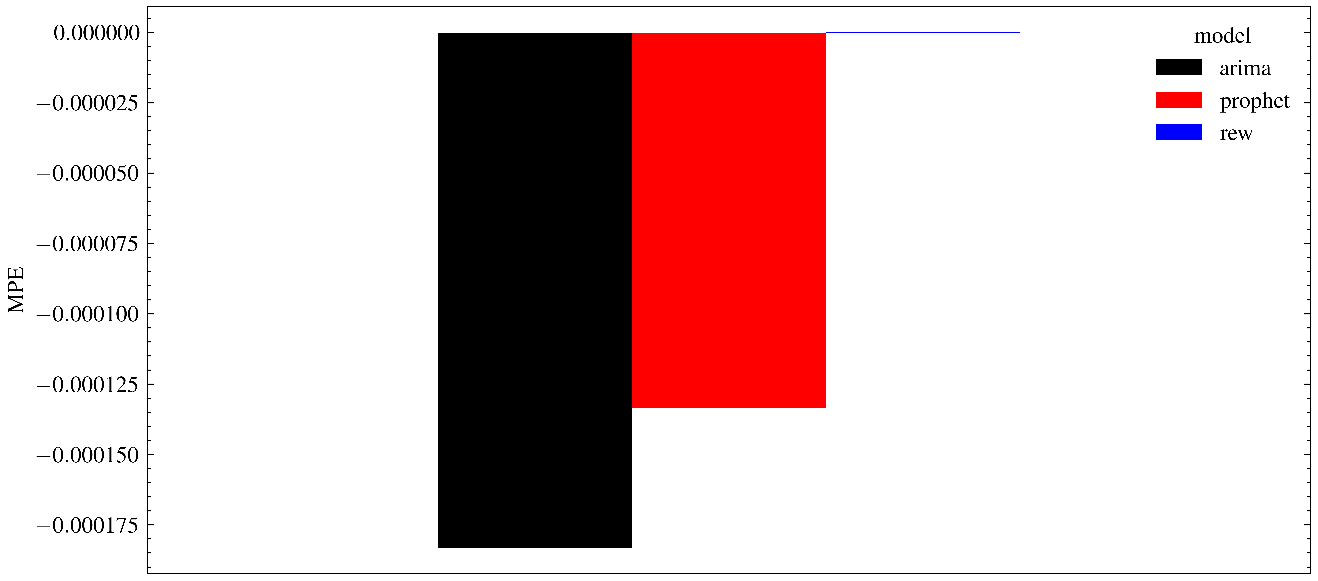
\includegraphics[width=5.0in]{img/temperatures_mpe_comparison.pdf}
    \caption{MPE por modelo para a temperatura diária de Melbourne}
\end{figure}

\begin{figure}[!htp]
    \centering
    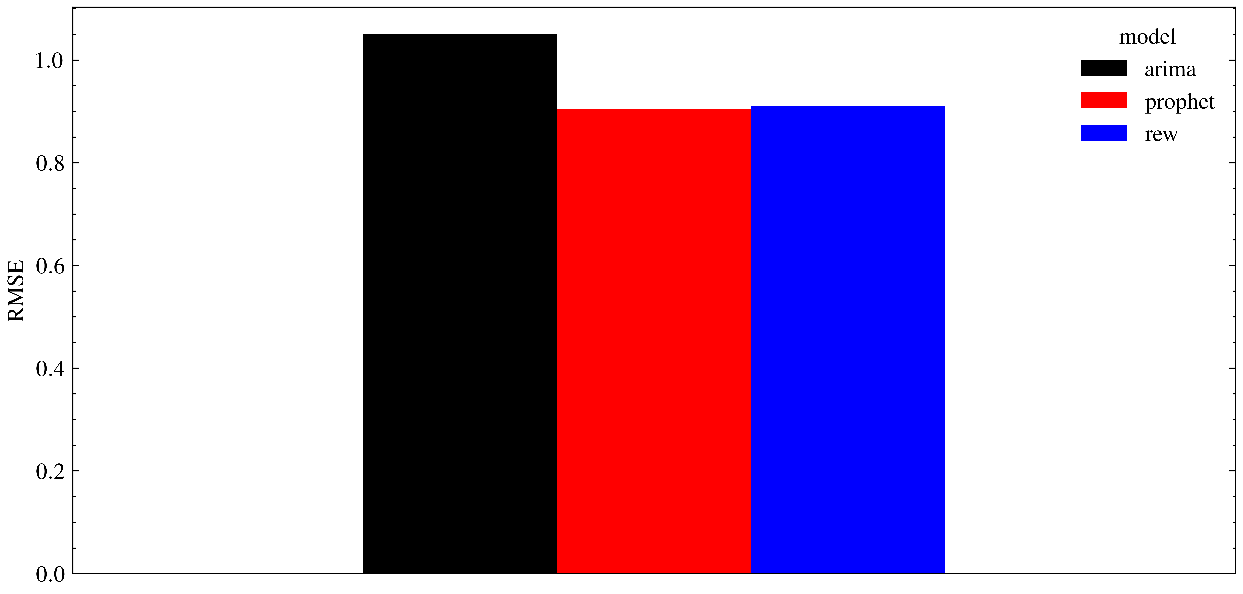
\includegraphics[width=5.0in]{img/temperatures_rmse_comparison.pdf}
    \caption{RMSE por modelo para a temperatura diária de Melbourne}
\end{figure}

\begin{figure}[!htp]
    \centering
    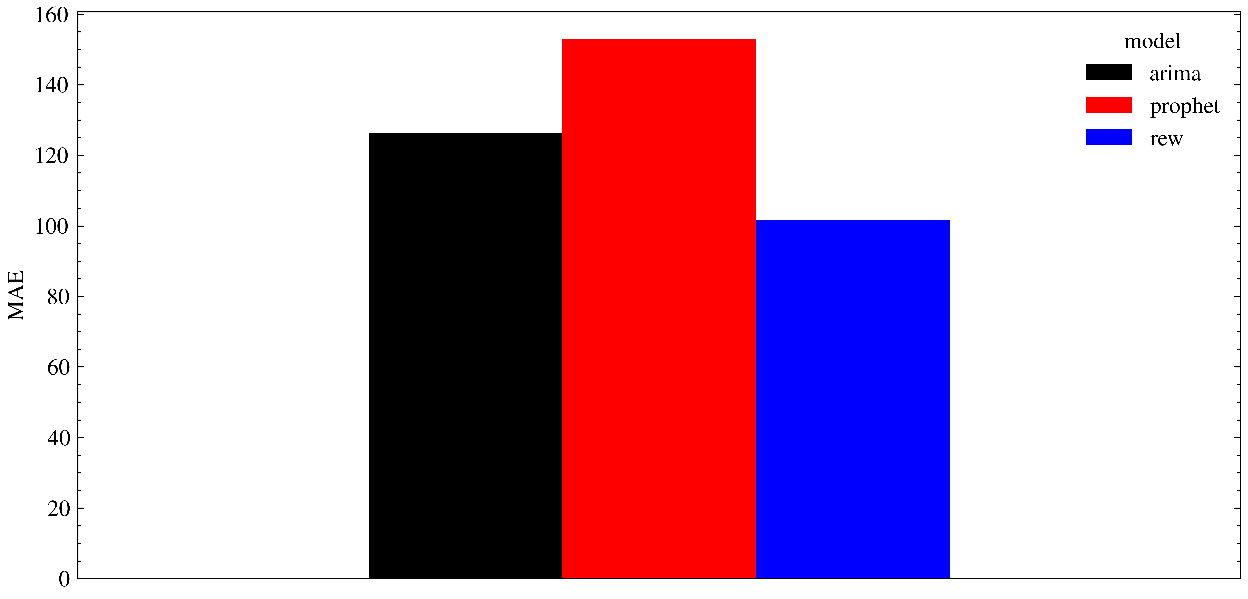
\includegraphics[width=5.0in]{img/synthetic_mae_comparison.pdf}
    \caption{MAE por modelo para os dados sintéticos.}
\end{figure}

\begin{figure}[!htp]
    \centering
    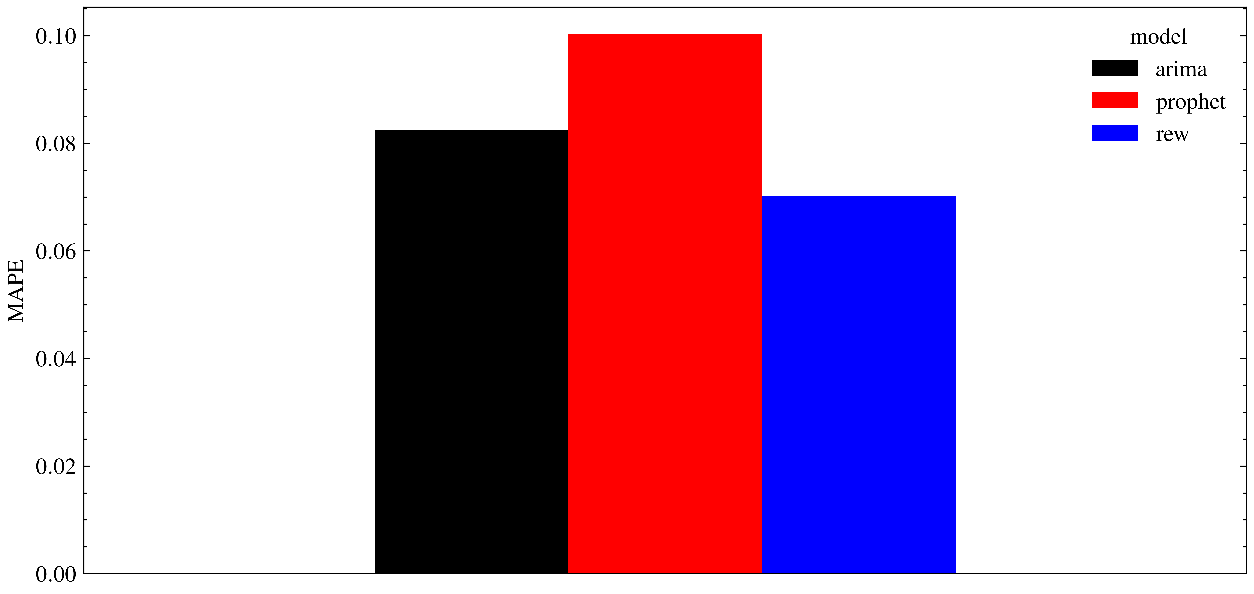
\includegraphics[width=5.0in]{img/synthetic_mape_comparison.pdf}
    \caption{MAPE por modelo para os dados sintéticos.}
\end{figure}

\begin{figure}[!htp]
    \centering
    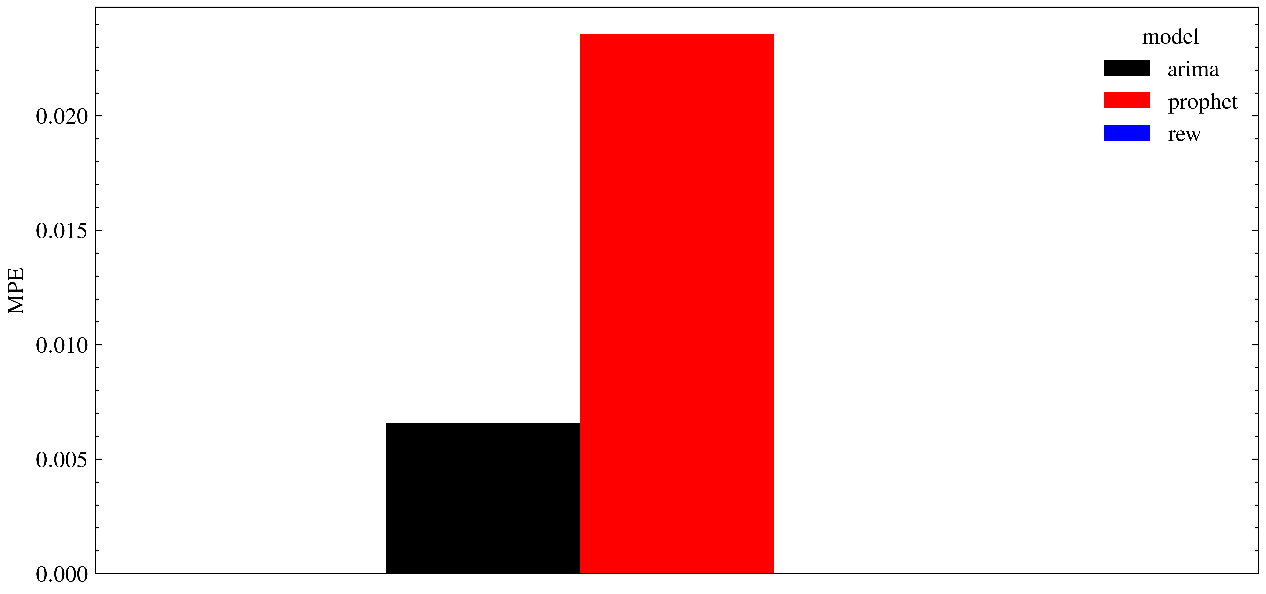
\includegraphics[width=5.0in]{img/synthetic_mpe_comparison.pdf}
    \caption{MPE por modelo para os dados sintéticos.}
\end{figure}

\begin{figure}[!htp]
    \centering
    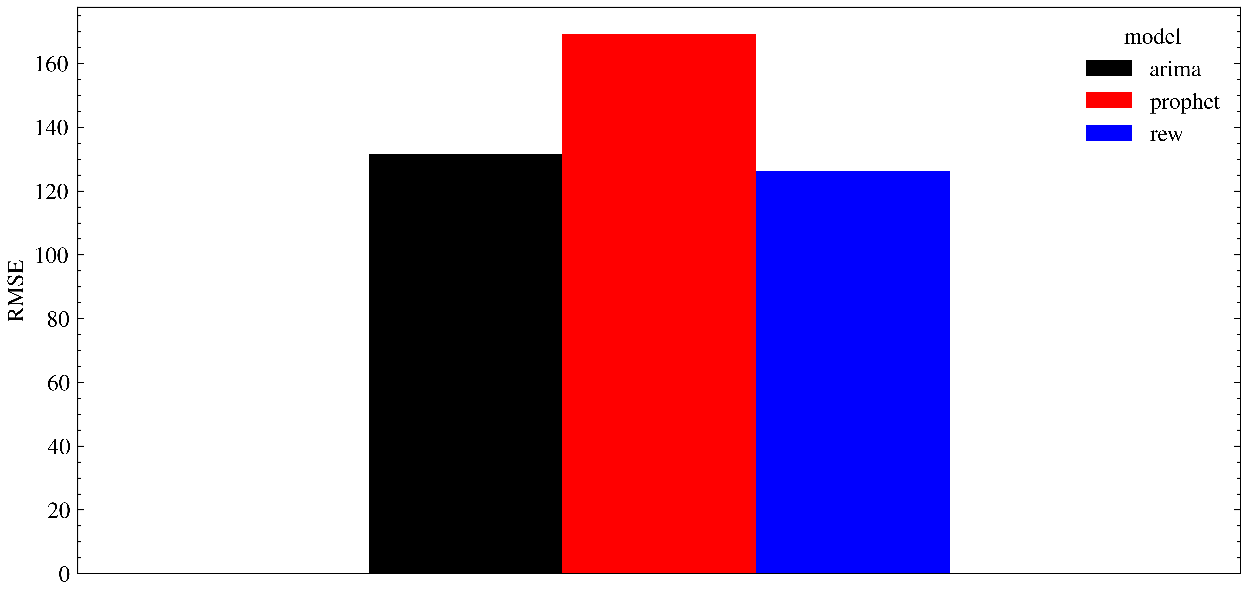
\includegraphics[width=5.0in]{img/synthetic_rmse_comparison.pdf}
    \caption{RMSE por modelo para os dados sintéticos.}
\end{figure}

\end{document}